\documentclass[a4paper,12pt]{article}

	%\usepackage[latin1]{inputenc}
	\usepackage[portuguese]{babel}

    \usepackage[breakable]{tcolorbox}
    \usepackage{parskip} % Stop auto-indenting (to mimic markdown behaviour)
    \usepackage{textgreek}

    
    
    \usepackage{iftex}
    \ifPDFTeX
    	\usepackage[T1]{fontenc}
    	\usepackage{mathpazo}
    \else
    	\usepackage{fontspec}
    \fi

    % Basic figure setup, for now with no caption control since it's done
    % automatically by Pandoc (which extracts ![](path) syntax from Markdown).
    \usepackage{graphicx}
    % Maintain compatibility with old templates. Remove in nbconvert 6.0
    \let\Oldincludegraphics\includegraphics
    % Ensure that by default, figures have no caption (until we provide a
    % proper Figure object with a Caption API and a way to capture that
    % in the conversion process - todo).
    \usepackage[justification=centering]{caption}
    %\DeclareCaptionFormat{nocaption}{}
    \captionsetup{aboveskip=0pt,belowskip=0pt}

    \usepackage{float}
    \floatplacement{figure}{H} % forces figures to be placed at the correct location
    \floatplacement{table}{H} % forces tables to be placed at the correct location
    \usepackage{xcolor} % Allow colors to be defined
    \usepackage{enumerate} % Needed for markdown enumerations to work
    \usepackage{geometry} % Used to adjust the document margins
    \usepackage{amsmath} % Equations
    \usepackage{amssymb} % Equations
    \usepackage{textcomp} % defines textquotesingle
    % Hack from http://tex.stackexchange.com/a/47451/13684:
    \AtBeginDocument{%
        \def\PYZsq{\textquotesingle}% Upright quotes in Pygmentized code
    }
    \usepackage{upquote} % Upright quotes for verbatim code
    \usepackage{eurosym} % defines \euro
    \usepackage[mathletters]{ucs} % Extended unicode (utf-8) support
    \usepackage{fancyvrb} % verbatim replacement that allows latex
    \usepackage{grffile} % extends the file name processing of package graphics 
                         % to support a larger range
    \makeatletter % fix for old versions of grffile with XeLaTeX
    \@ifpackagelater{grffile}{2019/11/01}
    {
      % Do nothing on new versions
    }
    {
      \def\Gread@@xetex#1{%
        \IfFileExists{"\Gin@base".bb}%
        {\Gread@eps{\Gin@base.bb}}%
        {\Gread@@xetex@aux#1}%
      }
    }
    \makeatother
    \usepackage[Export]{adjustbox} % Used to constrain images to a maximum size
    \adjustboxset{max size={0.9\linewidth}{0.9\paperheight}}

    % The hyperref package gives us a pdf with properly built
    % internal navigation ('pdf bookmarks' for the table of contents,
    % internal cross-reference links, web links for URLs, etc.)
    \usepackage{hyperref}
    % The default LaTeX title has an obnoxious amount of whitespace. By default,
    % titling removes some of it. It also provides customization options.
    \usepackage{titling}
    \usepackage{longtable} % longtable support required by pandoc >1.10
    \usepackage{booktabs}  % table support for pandoc > 1.12.2
    \usepackage[inline]{enumitem} % IRkernel/repr support (it uses the enumerate* environment)
    \usepackage[normalem]{ulem} % ulem is needed to support strikethroughs (\sout)
                                % normalem makes italics be italics, not underlines
    \usepackage{mathrsfs}
    

    
    % Colors for the hyperref package
    \definecolor{urlcolor}{rgb}{0,0,0} %{0,0,0.5} é azul escuro
    \definecolor{linkcolor}{rgb}{0,0,0}
    \definecolor{citecolor}{rgb}{0,0,0}

    % ANSI colors
    \definecolor{ansi-black}{HTML}{3E424D}
    \definecolor{ansi-black-intense}{HTML}{282C36}
    \definecolor{ansi-red}{HTML}{E75C58}
    \definecolor{ansi-red-intense}{HTML}{B22B31}
    \definecolor{ansi-green}{HTML}{00A250}
    \definecolor{ansi-green-intense}{HTML}{007427}
    \definecolor{ansi-yellow}{HTML}{DDB62B}
    \definecolor{ansi-yellow-intense}{HTML}{B27D12}
    \definecolor{ansi-blue}{HTML}{208FFB}
    \definecolor{ansi-blue-intense}{HTML}{0065CA}
    \definecolor{ansi-magenta}{HTML}{D160C4}
    \definecolor{ansi-magenta-intense}{HTML}{A03196}
    \definecolor{ansi-cyan}{HTML}{60C6C8}
    \definecolor{ansi-cyan-intense}{HTML}{258F8F}
    \definecolor{ansi-white}{HTML}{C5C1B4}
    \definecolor{ansi-white-intense}{HTML}{A1A6B2}
    \definecolor{ansi-default-inverse-fg}{HTML}{FFFFFF}
    \definecolor{ansi-default-inverse-bg}{HTML}{000000}

    % common color for the border for error outputs.
    \definecolor{outerrorbackground}{HTML}{FFDFDF}

    % commands and environments needed by pandoc snippets
    % extracted from the output of `pandoc -s`
    \providecommand{\tightlist}{%
      \setlength{\itemsep}{0pt}\setlength{\parskip}{0pt}}
    \DefineVerbatimEnvironment{Highlighting}{Verbatim}{commandchars=\\\{\}}
    % Add ',fontsize=\small' for more characters per line
    \newenvironment{Shaded}{}{}
    \newcommand{\KeywordTok}[1]{\textcolor[rgb]{0.00,0.44,0.13}{\textbf{{#1}}}}
    \newcommand{\DataTypeTok}[1]{\textcolor[rgb]{0.56,0.13,0.00}{{#1}}}
    \newcommand{\DecValTok}[1]{\textcolor[rgb]{0.25,0.63,0.44}{{#1}}}
    \newcommand{\BaseNTok}[1]{\textcolor[rgb]{0.25,0.63,0.44}{{#1}}}
    \newcommand{\FloatTok}[1]{\textcolor[rgb]{0.25,0.63,0.44}{{#1}}}
    \newcommand{\CharTok}[1]{\textcolor[rgb]{0.25,0.44,0.63}{{#1}}}
    \newcommand{\StringTok}[1]{\textcolor[rgb]{0.25,0.44,0.63}{{#1}}}
    \newcommand{\CommentTok}[1]{\textcolor[rgb]{0.38,0.63,0.69}{\textit{{#1}}}}
    \newcommand{\OtherTok}[1]{\textcolor[rgb]{0.00,0.44,0.13}{{#1}}}
    \newcommand{\AlertTok}[1]{\textcolor[rgb]{1.00,0.00,0.00}{\textbf{{#1}}}}
    \newcommand{\FunctionTok}[1]{\textcolor[rgb]{0.02,0.16,0.49}{{#1}}}
    \newcommand{\RegionMarkerTok}[1]{{#1}}
    \newcommand{\ErrorTok}[1]{\textcolor[rgb]{1.00,0.00,0.00}{\textbf{{#1}}}}
    \newcommand{\NormalTok}[1]{{#1}}
    
    % Additional commands for more recent versions of Pandoc
    \newcommand{\ConstantTok}[1]{\textcolor[rgb]{0.53,0.00,0.00}{{#1}}}
    \newcommand{\SpecialCharTok}[1]{\textcolor[rgb]{0.25,0.44,0.63}{{#1}}}
    \newcommand{\VerbatimStringTok}[1]{\textcolor[rgb]{0.25,0.44,0.63}{{#1}}}
    \newcommand{\SpecialStringTok}[1]{\textcolor[rgb]{0.73,0.40,0.53}{{#1}}}
    \newcommand{\ImportTok}[1]{{#1}}
    \newcommand{\DocumentationTok}[1]{\textcolor[rgb]{0.73,0.13,0.13}{\textit{{#1}}}}
    \newcommand{\AnnotationTok}[1]{\textcolor[rgb]{0.38,0.63,0.69}{\textbf{\textit{{#1}}}}}
    \newcommand{\CommentVarTok}[1]{\textcolor[rgb]{0.38,0.63,0.69}{\textbf{\textit{{#1}}}}}
    \newcommand{\VariableTok}[1]{\textcolor[rgb]{0.10,0.09,0.49}{{#1}}}
    \newcommand{\ControlFlowTok}[1]{\textcolor[rgb]{0.00,0.44,0.13}{\textbf{{#1}}}}
    \newcommand{\OperatorTok}[1]{\textcolor[rgb]{0.40,0.40,0.40}{{#1}}}
    \newcommand{\BuiltInTok}[1]{{#1}}
    \newcommand{\ExtensionTok}[1]{{#1}}
    \newcommand{\PreprocessorTok}[1]{\textcolor[rgb]{0.74,0.48,0.00}{{#1}}}
    \newcommand{\AttributeTok}[1]{\textcolor[rgb]{0.49,0.56,0.16}{{#1}}}
    \newcommand{\InformationTok}[1]{\textcolor[rgb]{0.38,0.63,0.69}{\textbf{\textit{{#1}}}}}
    \newcommand{\WarningTok}[1]{\textcolor[rgb]{0.38,0.63,0.69}{\textbf{\textit{{#1}}}}}
    
    
    % Define a nice break command that doesn't care if a line doesn't already
    % exist.
    \def\br{\hspace*{\fill} \\* }
    % Math Jax compatibility definitions
    \def\gt{>}
    \def\lt{<}
    \let\Oldtex\TeX
    \let\Oldlatex\LaTeX
    \renewcommand{\TeX}{\textrm{\Oldtex}}
    \renewcommand{\LaTeX}{\textrm{\Oldlatex}}
   
    
    
    
    
    
% Pygments definitions
\makeatletter
\def\PY@reset{\let\PY@it=\relax \let\PY@bf=\relax%
    \let\PY@ul=\relax \let\PY@tc=\relax%
    \let\PY@bc=\relax \let\PY@ff=\relax}
\def\PY@tok#1{\csname PY@tok@#1\endcsname}
\def\PY@toks#1+{\ifx\relax#1\empty\else%
    \PY@tok{#1}\expandafter\PY@toks\fi}
\def\PY@do#1{\PY@bc{\PY@tc{\PY@ul{%
    \PY@it{\PY@bf{\PY@ff{#1}}}}}}}
\def\PY#1#2{\PY@reset\PY@toks#1+\relax+\PY@do{#2}}

\expandafter\def\csname PY@tok@w\endcsname{\def\PY@tc##1{\textcolor[rgb]{0.73,0.73,0.73}{##1}}}
\expandafter\def\csname PY@tok@c\endcsname{\let\PY@it=\textit\def\PY@tc##1{\textcolor[rgb]{0.25,0.50,0.50}{##1}}}
\expandafter\def\csname PY@tok@cp\endcsname{\def\PY@tc##1{\textcolor[rgb]{0.74,0.48,0.00}{##1}}}
\expandafter\def\csname PY@tok@k\endcsname{\let\PY@bf=\textbf\def\PY@tc##1{\textcolor[rgb]{0.00,0.50,0.00}{##1}}}
\expandafter\def\csname PY@tok@kp\endcsname{\def\PY@tc##1{\textcolor[rgb]{0.00,0.50,0.00}{##1}}}
\expandafter\def\csname PY@tok@kt\endcsname{\def\PY@tc##1{\textcolor[rgb]{0.69,0.00,0.25}{##1}}}
\expandafter\def\csname PY@tok@o\endcsname{\def\PY@tc##1{\textcolor[rgb]{0.40,0.40,0.40}{##1}}}
\expandafter\def\csname PY@tok@ow\endcsname{\let\PY@bf=\textbf\def\PY@tc##1{\textcolor[rgb]{0.67,0.13,1.00}{##1}}}
\expandafter\def\csname PY@tok@nb\endcsname{\def\PY@tc##1{\textcolor[rgb]{0.00,0.50,0.00}{##1}}}
\expandafter\def\csname PY@tok@nf\endcsname{\def\PY@tc##1{\textcolor[rgb]{0.00,0.00,1.00}{##1}}}
\expandafter\def\csname PY@tok@nc\endcsname{\let\PY@bf=\textbf\def\PY@tc##1{\textcolor[rgb]{0.00,0.00,1.00}{##1}}}
\expandafter\def\csname PY@tok@nn\endcsname{\let\PY@bf=\textbf\def\PY@tc##1{\textcolor[rgb]{0.00,0.00,1.00}{##1}}}
\expandafter\def\csname PY@tok@ne\endcsname{\let\PY@bf=\textbf\def\PY@tc##1{\textcolor[rgb]{0.82,0.25,0.23}{##1}}}
\expandafter\def\csname PY@tok@nv\endcsname{\def\PY@tc##1{\textcolor[rgb]{0.10,0.09,0.49}{##1}}}
\expandafter\def\csname PY@tok@no\endcsname{\def\PY@tc##1{\textcolor[rgb]{0.53,0.00,0.00}{##1}}}
\expandafter\def\csname PY@tok@nl\endcsname{\def\PY@tc##1{\textcolor[rgb]{0.63,0.63,0.00}{##1}}}
\expandafter\def\csname PY@tok@ni\endcsname{\let\PY@bf=\textbf\def\PY@tc##1{\textcolor[rgb]{0.60,0.60,0.60}{##1}}}
\expandafter\def\csname PY@tok@na\endcsname{\def\PY@tc##1{\textcolor[rgb]{0.49,0.56,0.16}{##1}}}
\expandafter\def\csname PY@tok@nt\endcsname{\let\PY@bf=\textbf\def\PY@tc##1{\textcolor[rgb]{0.00,0.50,0.00}{##1}}}
\expandafter\def\csname PY@tok@nd\endcsname{\def\PY@tc##1{\textcolor[rgb]{0.67,0.13,1.00}{##1}}}
\expandafter\def\csname PY@tok@s\endcsname{\def\PY@tc##1{\textcolor[rgb]{0.73,0.13,0.13}{##1}}}
\expandafter\def\csname PY@tok@sd\endcsname{\let\PY@it=\textit\def\PY@tc##1{\textcolor[rgb]{0.73,0.13,0.13}{##1}}}
\expandafter\def\csname PY@tok@si\endcsname{\let\PY@bf=\textbf\def\PY@tc##1{\textcolor[rgb]{0.73,0.40,0.53}{##1}}}
\expandafter\def\csname PY@tok@se\endcsname{\let\PY@bf=\textbf\def\PY@tc##1{\textcolor[rgb]{0.73,0.40,0.13}{##1}}}
\expandafter\def\csname PY@tok@sr\endcsname{\def\PY@tc##1{\textcolor[rgb]{0.73,0.40,0.53}{##1}}}
\expandafter\def\csname PY@tok@ss\endcsname{\def\PY@tc##1{\textcolor[rgb]{0.10,0.09,0.49}{##1}}}
\expandafter\def\csname PY@tok@sx\endcsname{\def\PY@tc##1{\textcolor[rgb]{0.00,0.50,0.00}{##1}}}
\expandafter\def\csname PY@tok@m\endcsname{\def\PY@tc##1{\textcolor[rgb]{0.40,0.40,0.40}{##1}}}
\expandafter\def\csname PY@tok@gh\endcsname{\let\PY@bf=\textbf\def\PY@tc##1{\textcolor[rgb]{0.00,0.00,0.50}{##1}}}
\expandafter\def\csname PY@tok@gu\endcsname{\let\PY@bf=\textbf\def\PY@tc##1{\textcolor[rgb]{0.50,0.00,0.50}{##1}}}
\expandafter\def\csname PY@tok@gd\endcsname{\def\PY@tc##1{\textcolor[rgb]{0.63,0.00,0.00}{##1}}}
\expandafter\def\csname PY@tok@gi\endcsname{\def\PY@tc##1{\textcolor[rgb]{0.00,0.63,0.00}{##1}}}
\expandafter\def\csname PY@tok@gr\endcsname{\def\PY@tc##1{\textcolor[rgb]{1.00,0.00,0.00}{##1}}}
\expandafter\def\csname PY@tok@ge\endcsname{\let\PY@it=\textit}
\expandafter\def\csname PY@tok@gs\endcsname{\let\PY@bf=\textbf}
\expandafter\def\csname PY@tok@gp\endcsname{\let\PY@bf=\textbf\def\PY@tc##1{\textcolor[rgb]{0.00,0.00,0.50}{##1}}}
\expandafter\def\csname PY@tok@go\endcsname{\def\PY@tc##1{\textcolor[rgb]{0.53,0.53,0.53}{##1}}}
\expandafter\def\csname PY@tok@gt\endcsname{\def\PY@tc##1{\textcolor[rgb]{0.00,0.27,0.87}{##1}}}
\expandafter\def\csname PY@tok@err\endcsname{\def\PY@bc##1{\setlength{\fboxsep}{0pt}\fcolorbox[rgb]{1.00,0.00,0.00}{1,1,1}{\strut ##1}}}
\expandafter\def\csname PY@tok@kc\endcsname{\let\PY@bf=\textbf\def\PY@tc##1{\textcolor[rgb]{0.00,0.50,0.00}{##1}}}
\expandafter\def\csname PY@tok@kd\endcsname{\let\PY@bf=\textbf\def\PY@tc##1{\textcolor[rgb]{0.00,0.50,0.00}{##1}}}
\expandafter\def\csname PY@tok@kn\endcsname{\let\PY@bf=\textbf\def\PY@tc##1{\textcolor[rgb]{0.00,0.50,0.00}{##1}}}
\expandafter\def\csname PY@tok@kr\endcsname{\let\PY@bf=\textbf\def\PY@tc##1{\textcolor[rgb]{0.00,0.50,0.00}{##1}}}
\expandafter\def\csname PY@tok@bp\endcsname{\def\PY@tc##1{\textcolor[rgb]{0.00,0.50,0.00}{##1}}}
\expandafter\def\csname PY@tok@fm\endcsname{\def\PY@tc##1{\textcolor[rgb]{0.00,0.00,1.00}{##1}}}
\expandafter\def\csname PY@tok@vc\endcsname{\def\PY@tc##1{\textcolor[rgb]{0.10,0.09,0.49}{##1}}}
\expandafter\def\csname PY@tok@vg\endcsname{\def\PY@tc##1{\textcolor[rgb]{0.10,0.09,0.49}{##1}}}
\expandafter\def\csname PY@tok@vi\endcsname{\def\PY@tc##1{\textcolor[rgb]{0.10,0.09,0.49}{##1}}}
\expandafter\def\csname PY@tok@vm\endcsname{\def\PY@tc##1{\textcolor[rgb]{0.10,0.09,0.49}{##1}}}
\expandafter\def\csname PY@tok@sa\endcsname{\def\PY@tc##1{\textcolor[rgb]{0.73,0.13,0.13}{##1}}}
\expandafter\def\csname PY@tok@sb\endcsname{\def\PY@tc##1{\textcolor[rgb]{0.73,0.13,0.13}{##1}}}
\expandafter\def\csname PY@tok@sc\endcsname{\def\PY@tc##1{\textcolor[rgb]{0.73,0.13,0.13}{##1}}}
\expandafter\def\csname PY@tok@dl\endcsname{\def\PY@tc##1{\textcolor[rgb]{0.73,0.13,0.13}{##1}}}
\expandafter\def\csname PY@tok@s2\endcsname{\def\PY@tc##1{\textcolor[rgb]{0.73,0.13,0.13}{##1}}}
\expandafter\def\csname PY@tok@sh\endcsname{\def\PY@tc##1{\textcolor[rgb]{0.73,0.13,0.13}{##1}}}
\expandafter\def\csname PY@tok@s1\endcsname{\def\PY@tc##1{\textcolor[rgb]{0.73,0.13,0.13}{##1}}}
\expandafter\def\csname PY@tok@mb\endcsname{\def\PY@tc##1{\textcolor[rgb]{0.40,0.40,0.40}{##1}}}
\expandafter\def\csname PY@tok@mf\endcsname{\def\PY@tc##1{\textcolor[rgb]{0.40,0.40,0.40}{##1}}}
\expandafter\def\csname PY@tok@mh\endcsname{\def\PY@tc##1{\textcolor[rgb]{0.40,0.40,0.40}{##1}}}
\expandafter\def\csname PY@tok@mi\endcsname{\def\PY@tc##1{\textcolor[rgb]{0.40,0.40,0.40}{##1}}}
\expandafter\def\csname PY@tok@il\endcsname{\def\PY@tc##1{\textcolor[rgb]{0.40,0.40,0.40}{##1}}}
\expandafter\def\csname PY@tok@mo\endcsname{\def\PY@tc##1{\textcolor[rgb]{0.40,0.40,0.40}{##1}}}
\expandafter\def\csname PY@tok@ch\endcsname{\let\PY@it=\textit\def\PY@tc##1{\textcolor[rgb]{0.25,0.50,0.50}{##1}}}
\expandafter\def\csname PY@tok@cm\endcsname{\let\PY@it=\textit\def\PY@tc##1{\textcolor[rgb]{0.25,0.50,0.50}{##1}}}
\expandafter\def\csname PY@tok@cpf\endcsname{\let\PY@it=\textit\def\PY@tc##1{\textcolor[rgb]{0.25,0.50,0.50}{##1}}}
\expandafter\def\csname PY@tok@c1\endcsname{\let\PY@it=\textit\def\PY@tc##1{\textcolor[rgb]{0.25,0.50,0.50}{##1}}}
\expandafter\def\csname PY@tok@cs\endcsname{\let\PY@it=\textit\def\PY@tc##1{\textcolor[rgb]{0.25,0.50,0.50}{##1}}}

\def\PYZbs{\char`\\}
\def\PYZus{\char`\_}
\def\PYZob{\char`\{}
\def\PYZcb{\char`\}}
\def\PYZca{\char`\^}
\def\PYZam{\char`\&}
\def\PYZlt{\char`\<}
\def\PYZgt{\char`\>}
\def\PYZsh{\char`\#}
\def\PYZpc{\char`\%}
\def\PYZdl{\char`\$}
\def\PYZhy{\char`\-}
\def\PYZsq{\char`\'}
\def\PYZdq{\char`\"}
\def\PYZti{\char`\~}
% for compatibility with earlier versions
\def\PYZat{@}
\def\PYZlb{[}
\def\PYZrb{]}
\makeatother


    % For linebreaks inside Verbatim environment from package fancyvrb. 
    \makeatletter
        \newbox\Wrappedcontinuationbox 
        \newbox\Wrappedvisiblespacebox 
        \newcommand*\Wrappedvisiblespace {\textcolor{red}{\textvisiblespace}} 
        \newcommand*\Wrappedcontinuationsymbol {\textcolor{red}{\llap{\tiny$\m@th\hookrightarrow$}}} 
        \newcommand*\Wrappedcontinuationindent {3ex } 
        \newcommand*\Wrappedafterbreak {\kern\Wrappedcontinuationindent\copy\Wrappedcontinuationbox} 
        % Take advantage of the already applied Pygments mark-up to insert 
        % potential linebreaks for TeX processing. 
        %        {, <, #, %, $, ' and ": go to next line. 
        %        _, }, ^, &, >, - and ~: stay at end of broken line. 
        % Use of \textquotesingle for straight quote. 
        \newcommand*\Wrappedbreaksatspecials {% 
            \def\PYGZus{\discretionary{\char`\_}{\Wrappedafterbreak}{\char`\_}}% 
            \def\PYGZob{\discretionary{}{\Wrappedafterbreak\char`\{}{\char`\{}}% 
            \def\PYGZcb{\discretionary{\char`\}}{\Wrappedafterbreak}{\char`\}}}% 
            \def\PYGZca{\discretionary{\char`\^}{\Wrappedafterbreak}{\char`\^}}% 
            \def\PYGZam{\discretionary{\char`\&}{\Wrappedafterbreak}{\char`\&}}% 
            \def\PYGZlt{\discretionary{}{\Wrappedafterbreak\char`\<}{\char`\<}}% 
            \def\PYGZgt{\discretionary{\char`\>}{\Wrappedafterbreak}{\char`\>}}% 
            \def\PYGZsh{\discretionary{}{\Wrappedafterbreak\char`\#}{\char`\#}}% 
            \def\PYGZpc{\discretionary{}{\Wrappedafterbreak\char`\%}{\char`\%}}% 
            \def\PYGZdl{\discretionary{}{\Wrappedafterbreak\char`\$}{\char`\$}}% 
            \def\PYGZhy{\discretionary{\char`\-}{\Wrappedafterbreak}{\char`\-}}% 
            \def\PYGZsq{\discretionary{}{\Wrappedafterbreak\textquotesingle}{\textquotesingle}}% 
            \def\PYGZdq{\discretionary{}{\Wrappedafterbreak\char`\"}{\char`\"}}% 
            \def\PYGZti{\discretionary{\char`\~}{\Wrappedafterbreak}{\char`\~}}% 
        } 
        % Some characters . , ; ? ! / are not pygmentized. 
        % This macro makes them "active" and they will insert potential linebreaks 
        \newcommand*\Wrappedbreaksatpunct {% 
            \lccode`\~`\.\lowercase{\def~}{\discretionary{\hbox{\char`\.}}{\Wrappedafterbreak}{\hbox{\char`\.}}}% 
            \lccode`\~`\,\lowercase{\def~}{\discretionary{\hbox{\char`\,}}{\Wrappedafterbreak}{\hbox{\char`\,}}}% 
            \lccode`\~`\;\lowercase{\def~}{\discretionary{\hbox{\char`\;}}{\Wrappedafterbreak}{\hbox{\char`\;}}}% 
            \lccode`\~`\:\lowercase{\def~}{\discretionary{\hbox{\char`\:}}{\Wrappedafterbreak}{\hbox{\char`\:}}}% 
            \lccode`\~`\?\lowercase{\def~}{\discretionary{\hbox{\char`\?}}{\Wrappedafterbreak}{\hbox{\char`\?}}}% 
            \lccode`\~`\!\lowercase{\def~}{\discretionary{\hbox{\char`\!}}{\Wrappedafterbreak}{\hbox{\char`\!}}}% 
            \lccode`\~`\/\lowercase{\def~}{\discretionary{\hbox{\char`\/}}{\Wrappedafterbreak}{\hbox{\char`\/}}}% 
            \catcode`\.\active
            \catcode`\,\active 
            \catcode`\;\active
            \catcode`\:\active
            \catcode`\?\active
            \catcode`\!\active
            \catcode`\/\active 
            \lccode`\~`\~ 	
        }
    \makeatother

    \let\OriginalVerbatim=\Verbatim
    \makeatletter
    \renewcommand{\Verbatim}[1][1]{%
    	
    	%\fontfamily{fi4}
  		%\fontsize{11}{2}
  		\linespread{0.9}	
    	
        %\parskip\z@skip
        \sbox\Wrappedcontinuationbox {\Wrappedcontinuationsymbol}%
        \sbox\Wrappedvisiblespacebox {\FV@SetupFont\Wrappedvisiblespace}%
        \def\FancyVerbFormatLine ##1{\hsize\linewidth
            \vtop{\raggedright\hyphenpenalty\z@\exhyphenpenalty\z@
                \doublehyphendemerits\z@\finalhyphendemerits\z@
                \strut ##1\strut}%
        }%
        % If the linebreak is at a space, the latter will be displayed as visible
        % space at end of first line, and a continuation symbol starts next line.
        % Stretch/shrink are however usually zero for typewriter font.
        \def\FV@Space {%
            \nobreak\hskip\z@ plus\fontdimen3\font minus\fontdimen4\font
            \discretionary{\copy\Wrappedvisiblespacebox}{\Wrappedafterbreak}
            {\kern\fontdimen2\font}%
        }%
        
        % Allow breaks at special characters using \PYG... macros.
        \Wrappedbreaksatspecials
        % Breaks at punctuation characters . , ; ? ! and / need catcode=\active 	
        \OriginalVerbatim[#1,codes*=\Wrappedbreaksatpunct]%
    }
    \makeatother

    % Exact colors from NB
    \definecolor{incolor}{HTML}{303F9F}
    \definecolor{outcolor}{HTML}{D84315}
    \definecolor{cellborder}{HTML}{CFCFCF}
    \definecolor{cellbackground}{HTML}{F7F7F7}
    
    % prompt
    \makeatletter
    \newcommand{\boxspacing}{\kern\kvtcb@left@rule\kern\kvtcb@boxsep}
    \makeatother
    \newcommand{\prompt}[4]{ }
    

    
    % Prevent overflowing lines due to hard-to-break entities
    \sloppy 
    % Setup hyperref package
    \hypersetup{
      breaklinks=true,  % so long urls are correctly broken across lines
      colorlinks=true,
      urlcolor=urlcolor,
      linkcolor=linkcolor,
      citecolor=citecolor,
      }
    % Slightly bigger margins than the latex defaults
    
    \geometry{verbose,tmargin=1in,bmargin=1in,lmargin=1in,rmargin=1in}

 \linespread{1.25}
    
 
 \makeatletter
 
 \newcommand{\subtitle}[1]{\def\@subtitle{#1}}
 
 \renewcommand\maketitle{%
 		\begin{center}
 			{\large Universidade Federal do Rio Grande do Sul}\\
 			{\normalsize Escola de Engenharia}\\
 			{\normalsize Programa de Pós-Graduação em Engenharia Civil}\\[48pt] 
 			{\Large \@title }\\[8pt] 
 			{\large \@subtitle }\\[24pt] 
 		\end{center}
 		\begin{flushright}
 			{\normalsize \@author}\\[24pt] 
 		\end{flushright}
 		\begin{center}
 			{\@date}\\[0pt] 
 		\end{center}
 		\noindent\rule{17cm}{0.8pt}
 }
\makeatother

\author{Eduardo Pagnussat Titello}
\title{PEC00144 - Métodos Experimentais em Engenharia Civil}
\subtitle{Trabalho final}
\date{Fevereiro de 2021}


\begin{document}
	
\maketitle

Este trabalho consiste em projetar, construir e instrumentar um modelo
reduzido. A estrutura adotada é uma torre de 3 pavimentos/níveis,
representada por um \emph{shear building}, e tem-se como objetivo a
determinação da frequência fundamental de vibração da estrutura real a
partir do modelo reduzido.

\tableofcontents

\pagebreak

    \begin{tcolorbox}[breakable, size=fbox, boxrule=1pt, pad at break*=1mm,colback=cellbackground, colframe=cellborder]
\prompt{In}{incolor}{1}{\boxspacing}
\begin{Verbatim}[commandchars=\\\{\}]
\PY{c+c1}{\PYZsh{} Importando e configurando módulos}
\PY{k+kn}{import} \PY{n+nn}{numpy} \PY{k}{as} \PY{n+nn}{np}
\PY{k+kn}{import} \PY{n+nn}{pandas} \PY{k}{as} \PY{n+nn}{pd} 
\PY{k+kn}{import} \PY{n+nn}{matplotlib}\PY{n+nn}{.}\PY{n+nn}{pyplot} \PY{k}{as} \PY{n+nn}{plt}
\PY{o}{\PYZpc{}}\PY{k}{config} InlineBackend.figure\PYZus{}format = \PYZsq{}svg\PYZsq{}
\PY{k+kn}{import} \PY{n+nn}{jupyter2latex} \PY{k}{as} \PY{n+nn}{j2l}
\PY{k+kn}{import} \PY{n+nn}{scipy}\PY{n+nn}{.}\PY{n+nn}{linalg}
\PY{k+kn}{import} \PY{n+nn}{scipy}\PY{n+nn}{.}\PY{n+nn}{stats} \PY{k}{as} \PY{n+nn}{st}
\PY{k+kn}{from} \PY{n+nn}{MRPy} \PY{k+kn}{import} \PY{n}{MRPy}
\PY{k+kn}{import} \PY{n+nn}{serial}
\PY{k+kn}{import} \PY{n+nn}{time}
\end{Verbatim}
\end{tcolorbox}

    \hypertarget{apresentauxe7uxe3o-da-estrutura-real}{%
\section{Apresentação da estrutura
real}\label{apresentauxe7uxe3o-da-estrutura-real}}

A estrutura a ser representada pelo modelo é uma torre de planta
quadrada, formada por um pilar em cada extremidade e construída em
concreto C25. Essa e suas dimensões são apresentadas a seguir:

\begin{figure}
\centering
\includegraphics[scale=0.7]{../images/estrutura}
\caption{Estrutura}
\end{figure}

Adotando concreto da classe C25 tem-se \(E_C=28GPa\), transcrevendo as
propriedades da estrutura real tem-se:

    \begin{tcolorbox}[breakable, size=fbox, boxrule=1pt, pad at break*=1mm,colback=cellbackground, colframe=cellborder]
\prompt{In}{incolor}{2}{\boxspacing}
\begin{Verbatim}[commandchars=\\\{\}]
\PY{c+c1}{\PYZsh{} Dados da geometria}
\PY{n}{est\PYZus{}L}  \PY{o}{=} \PY{l+m+mf}{5.0}            \PY{c+c1}{\PYZsh{} Distância entre pisos}
\PY{n}{est\PYZus{}Pn} \PY{o}{=} \PY{l+m+mi}{4}              \PY{c+c1}{\PYZsh{} Pilares por pavimento}
\PY{n}{est\PYZus{}Pb} \PY{o}{=} \PY{l+m+mf}{0.25}           \PY{c+c1}{\PYZsh{} Largura dos pilares}
\PY{n}{est\PYZus{}Vn} \PY{o}{=} \PY{l+m+mi}{4}              \PY{c+c1}{\PYZsh{} Vigas por pavimento}
\PY{n}{est\PYZus{}Vb} \PY{o}{=} \PY{l+m+mf}{0.20}           \PY{c+c1}{\PYZsh{} Largura das vigas}
\PY{n}{est\PYZus{}Vh} \PY{o}{=} \PY{l+m+mf}{0.40}           \PY{c+c1}{\PYZsh{} Altura das vigas}
\PY{n}{est\PYZus{}LP} \PY{o}{=} \PY{l+m+mf}{4.00}           \PY{c+c1}{\PYZsh{} Lado dos pavimentos}
\PY{n}{est\PYZus{}Lh} \PY{o}{=} \PY{l+m+mf}{0.10}           \PY{c+c1}{\PYZsh{} Altura das lajes }
\PY{n}{est\PYZus{}cg} \PY{o}{=} \PY{l+m+mi}{335}            \PY{c+c1}{\PYZsh{} Carga nas lajes/m²}

\PY{c+c1}{\PYZsh{} Rigidez EI}
\PY{n}{est\PYZus{}I} \PY{o}{=} \PY{n}{est\PYZus{}Pb}\PY{o}{*}\PY{o}{*}\PY{l+m+mi}{4}\PY{o}{/}\PY{l+m+mi}{12}    \PY{c+c1}{\PYZsh{} Inércia do pilar}
\PY{n}{est\PYZus{}E} \PY{o}{=} \PY{l+m+mf}{28E9}            \PY{c+c1}{\PYZsh{} E do concreto}
\PY{n}{est\PYZus{}EI} \PY{o}{=} \PY{n}{est\PYZus{}I}\PY{o}{*}\PY{n}{est\PYZus{}E}    \PY{c+c1}{\PYZsh{} EI do pilar}
\end{Verbatim}
\end{tcolorbox}

    \hypertarget{projeto-do-modelo-reduzido}{%
\section{Projeto do modelo reduzido}\label{projeto-do-modelo-reduzido}}

O projeto do modelo reduzido é baseado na introdução de escalas que
relacionem as grandezas do modelo reduzido e do modelo real, onde o
número de escalas deve ser menor ou igual ao número de grandezas
fundamentais envolvidas no problema. Para o problema em questão as
grandezas fundamentais são três: comprimento (\(L\)), massa (\(M\)) e
tempo (\(T\)), que formam a base da matriz dimensional. Para construção
do modelo reduzido as grandezas escolhidas para serem escaladas são
relativas ao comprimento (\(L\)), à rigidez à flexão (\(EI\)) e à
aceleração (\(a\)).

    Os fatores de escala adotados para \(L\) e \(EI\) são baseados no
material empregado para construção das colunas do modelo, essas são
formadas por réguas de alumínio, com \(52.5 cm\) de comprimento,
\(2.58 cm\) de largura e \(0.10 cm\) de espessura, dimensões obtidas com
auxílio de um paquimetro. As réguas utilizadas são apresentadas na
figura a seguir:

\begin{figure}
\centering
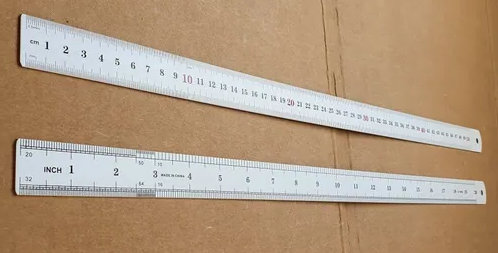
\includegraphics[scale=0.8]{../images/reguas.png}
\caption{Réguas}
\end{figure}

    \begin{tcolorbox}[breakable, size=fbox, boxrule=1pt, pad at break*=1mm,colback=cellbackground, colframe=cellborder]
\prompt{In}{incolor}{3}{\boxspacing}
\begin{Verbatim}[commandchars=\\\{\}]
\PY{n}{mod\PYZus{}b} \PY{o}{=} \PY{l+m+mf}{0.0258}
\PY{n}{mod\PYZus{}h} \PY{o}{=} \PY{l+m+mf}{0.0010}
\PY{n}{mod\PYZus{}E} \PY{o}{=} \PY{l+m+mf}{70E9}
\end{Verbatim}
\end{tcolorbox}

    Descontando um trecho para realização do engaste e dividindo o
comprimento restante da régua em 3 partes iguais, a distância entre os
pavimentos é representada por trechos de \(16.5 cm\), logo, a escala de
comprimento \(\lambda_L\) é:

    \begin{tcolorbox}[breakable, size=fbox, boxrule=1pt, pad at break*=1mm,colback=cellbackground, colframe=cellborder]
\prompt{In}{incolor}{4}{\boxspacing}
\begin{Verbatim}[commandchars=\\\{\}]
\PY{n}{mod\PYZus{}L} \PY{o}{=} \PY{l+m+mf}{0.165}
\PY{n}{scale\PYZus{}L} \PY{o}{=} \PY{n}{mod\PYZus{}L}\PY{o}{/}\PY{n}{est\PYZus{}L}

\PY{n}{j2l}\PY{o}{.}\PY{n}{print}\PY{p}{(}\PY{l+s+sa}{f}\PY{l+s+s2}{\PYZdq{}}\PY{l+s+s2}{Escala de comprimentos: \PYZdl{} }\PY{l+s+s2}{\PYZbs{}}\PY{l+s+s2}{lambda\PYZus{}L = 1:}\PY{l+s+si}{\PYZob{}}\PY{l+m+mi}{1}\PY{o}{/}\PY{n}{scale\PYZus{}L}\PY{l+s+si}{:}\PY{l+s+s2}{.2f}\PY{l+s+si}{\PYZcb{}}\PY{l+s+s2}{ \PYZdl{}.}\PY{l+s+s2}{\PYZdq{}}\PY{p}{)}
\end{Verbatim}
\end{tcolorbox}

    Escala de comprimentos: $ \lambda_L = 1:30.30 $.

    
    A escala da rigidez à flexão \(EI\) relaciona a rigidez das 2 réguas à
das 4 colunas da torre. Assumindo para as réguas \(E_{Al}=70 GPa\), a
rigidez \(EI\) das réguas e a escala de rigidez são dadas por:

    \begin{tcolorbox}[breakable, size=fbox, boxrule=1pt, pad at break*=1mm,colback=cellbackground, colframe=cellborder]
\prompt{In}{incolor}{5}{\boxspacing}
\begin{Verbatim}[commandchars=\\\{\}]
\PY{n}{mod\PYZus{}I} \PY{o}{=} \PY{n}{mod\PYZus{}b} \PY{o}{*} \PY{n}{mod\PYZus{}h}\PY{o}{*}\PY{o}{*}\PY{l+m+mi}{3} \PY{o}{/} \PY{l+m+mi}{12}
\PY{n}{mod\PYZus{}EI} \PY{o}{=} \PY{n}{mod\PYZus{}E}\PY{o}{*}\PY{n}{mod\PYZus{}I}
\PY{n}{scale\PYZus{}EI} \PY{o}{=} \PY{p}{(}\PY{l+m+mi}{2}\PY{o}{*}\PY{n}{mod\PYZus{}EI}\PY{p}{)}\PY{o}{/}\PY{p}{(}\PY{n}{est\PYZus{}Pn}\PY{o}{*}\PY{n}{est\PYZus{}EI}\PY{p}{)}

\PY{n}{j2l}\PY{o}{.}\PY{n}{print}\PY{p}{(}\PY{l+s+s1}{\PYZsq{}\PYZsq{}\PYZsq{}}\PY{l+s+s1}{\PYZhy{} Momento de inércia de uma régua: \PYZdl{}I=}\PY{l+s+si}{\PYZob{}mod\PYZus{}I:.3E\PYZcb{}}\PY{l+s+s1}{ }\PY{l+s+s1}{\PYZbs{}}\PY{l+s+s1}{: m\PYZca{}4\PYZdl{}}

\PY{l+s+s1}{\PYZhy{} Rigidez à flexão de uma régua: \PYZdl{}EI = }\PY{l+s+si}{\PYZob{}mod\PYZus{}EI:.3E\PYZcb{}}\PY{l+s+s1}{ Nm\PYZca{}2\PYZdl{}}

\PY{l+s+s1}{\PYZhy{} Escala de rigidez: \PYZdl{}}\PY{l+s+s1}{\PYZbs{}}\PY{l+s+s1}{lambda\PYZus{}}\PY{l+s+si}{\PYZob{}EI\PYZcb{}}\PY{l+s+s1}{=1:}\PY{l+s+si}{\PYZob{}scale\PYZus{}EI:.3E\PYZcb{}}\PY{l+s+s1}{ \PYZdl{}}
\PY{l+s+s1}{\PYZsq{}\PYZsq{}\PYZsq{}}\PY{o}{.}\PY{n}{format}\PY{p}{(}\PY{n}{mod\PYZus{}I}\PY{o}{=}\PY{n}{mod\PYZus{}I}\PY{p}{,} \PY{n}{mod\PYZus{}EI}\PY{o}{=}\PY{n}{mod\PYZus{}EI}\PY{p}{,} \PY{n}{EI}\PY{o}{=}\PY{l+s+s1}{\PYZsq{}}\PY{l+s+si}{\PYZob{}EI\PYZcb{}}\PY{l+s+s1}{\PYZsq{}}\PY{p}{,} \PY{n}{scale\PYZus{}EI}\PY{o}{=}\PY{l+m+mi}{1}\PY{o}{/}\PY{n}{scale\PYZus{}EI}\PY{p}{)}\PY{p}{)}
\end{Verbatim}
\end{tcolorbox}

    - Momento de inércia de uma régua: $I=2.150E-12 \: m^4$

- Rigidez à flexão de uma régua: $EI = 1.505E-01 Nm^2$

- Escala de rigidez: $\lambda_{EI}=1:1.211E+08 $


    
    Em relação à escala de acelerações (\(a\)) optou-se por manter a
proporção \(\lambda_a=1:1\). Todavia, visto que o problema de vibração
livre é independente da aceleração da gravidade essa poderia ser
alterada.

    \begin{tcolorbox}[breakable, size=fbox, boxrule=1pt, pad at break*=1mm,colback=cellbackground, colframe=cellborder]
\prompt{In}{incolor}{6}{\boxspacing}
\begin{Verbatim}[commandchars=\\\{\}]
\PY{n}{scale\PYZus{}a} \PY{o}{=} \PY{l+m+mi}{1}\PY{o}{/}\PY{l+m+mi}{1}
\end{Verbatim}
\end{tcolorbox}

    Em posse das escalas impostas, para construção do modelo reduzido e
realização da análise devem ser conhecidas as escalas derivadas
necessárias, que são obtidas através de uma análise dimensional, onde a
base da nova matriz dimensional será formada pelas grandezas \(L\),
\(EI\) e \(a\). Fazendo uso da metodologia implementada por Rocha
(2021), a base da matriz dimensional é alterada para a base \(L\),
\(EI\) e \(a\):

    \begin{tcolorbox}[breakable, size=fbox, boxrule=1pt, pad at break*=1mm,colback=cellbackground, colframe=cellborder]
\prompt{In}{incolor}{7}{\boxspacing}
\begin{Verbatim}[commandchars=\\\{\}]
\PY{c+c1}{\PYZsh{} Importando DimData }
\PY{n}{DimData} \PY{o}{=} \PY{n}{pd}\PY{o}{.}\PY{n}{read\PYZus{}excel}\PY{p}{(}\PY{l+s+s1}{\PYZsq{}}\PY{l+s+s1}{../Resources/DimData.xlsx}\PY{l+s+s1}{\PYZsq{}}\PY{p}{,} \PY{n}{index\PYZus{}col}\PY{o}{=}\PY{l+m+mi}{0}\PY{p}{,} \PY{n}{sheet\PYZus{}name}\PY{o}{=}\PY{l+s+s1}{\PYZsq{}}\PY{l+s+s1}{DimData}\PY{l+s+s1}{\PYZsq{}}\PY{p}{)}

\PY{c+c1}{\PYZsh{} Grandezas fundamentais originais }
\PY{n}{LMT} \PY{o}{=} \PY{p}{[}\PY{l+s+s1}{\PYZsq{}}\PY{l+s+s1}{L}\PY{l+s+s1}{\PYZsq{}}\PY{p}{,} \PY{l+s+s1}{\PYZsq{}}\PY{l+s+s1}{M}\PY{l+s+s1}{\PYZsq{}}\PY{p}{,} \PY{l+s+s1}{\PYZsq{}}\PY{l+s+s1}{T}\PY{l+s+s1}{\PYZsq{}}\PY{p}{]}

\PY{c+c1}{\PYZsh{} Novas base de grandezas}
\PY{n}{ABC} \PY{o}{=} \PY{p}{[}\PY{l+s+s1}{\PYZsq{}}\PY{l+s+s1}{L}\PY{l+s+s1}{\PYZsq{}}\PY{p}{,} \PY{l+s+s1}{\PYZsq{}}\PY{l+s+s1}{EI}\PY{l+s+s1}{\PYZsq{}}\PY{p}{,} \PY{l+s+s1}{\PYZsq{}}\PY{l+s+s1}{a}\PY{l+s+s1}{\PYZsq{}}\PY{p}{]} 

\PY{c+c1}{\PYZsh{} Importa matriz dimensional de ABC na base LMT}
\PY{n}{base} \PY{o}{=} \PY{n}{DimData}\PY{o}{.}\PY{n}{loc}\PY{p}{[}\PY{n}{ABC}\PY{p}{,} \PY{n}{LMT}\PY{p}{]}
\PY{n}{j2l}\PY{o}{.}\PY{n}{df2table}\PY{p}{(}\PY{n}{base}\PY{p}{,} \PY{l+s+s1}{\PYZsq{}}\PY{l+s+si}{\PYZob{}\PYZcb{}}\PY{l+s+s1}{ na base }\PY{l+s+si}{\PYZob{}\PYZcb{}}\PY{l+s+s1}{\PYZsq{}}\PY{o}{.}\PY{n}{format}\PY{p}{(}\PY{l+s+s1}{\PYZsq{}}\PY{l+s+s1}{,}\PY{l+s+s1}{\PYZsq{}}\PY{o}{.}\PY{n}{join}\PY{p}{(}\PY{n}{ABC}\PY{p}{)}\PY{p}{,} \PY{l+s+s1}{\PYZsq{}}\PY{l+s+s1}{,}\PY{l+s+s1}{\PYZsq{}}\PY{o}{.}\PY{n}{join}\PY{p}{(}\PY{n}{LMT}\PY{p}{)}\PY{p}{)}\PY{p}{)}

\PY{c+c1}{\PYZsh{} Inverte base de unidades de LMT para ABC}
\PY{n}{base\PYZus{}i} \PY{o}{=} \PY{n}{pd}\PY{o}{.}\PY{n}{DataFrame}\PY{p}{(}\PY{n}{np}\PY{o}{.}\PY{n}{linalg}\PY{o}{.}\PY{n}{inv}\PY{p}{(}\PY{n}{base}\PY{p}{)}\PY{p}{,} \PY{n}{index}\PY{o}{=}\PY{n}{LMT}\PY{p}{,} \PY{n}{columns}\PY{o}{=}\PY{n}{ABC}\PY{p}{)}
\PY{n}{j2l}\PY{o}{.}\PY{n}{df2table}\PY{p}{(}\PY{n}{base\PYZus{}i}\PY{p}{,} \PY{l+s+s1}{\PYZsq{}}\PY{l+s+si}{\PYZob{}\PYZcb{}}\PY{l+s+s1}{ na base }\PY{l+s+si}{\PYZob{}\PYZcb{}}\PY{l+s+s1}{\PYZsq{}}\PY{o}{.}\PY{n}{format}\PY{p}{(}\PY{l+s+s1}{\PYZsq{}}\PY{l+s+s1}{,}\PY{l+s+s1}{\PYZsq{}}\PY{o}{.}\PY{n}{join}\PY{p}{(}\PY{n}{LMT}\PY{p}{)}\PY{p}{,} \PY{l+s+s1}{\PYZsq{}}\PY{l+s+s1}{,}\PY{l+s+s1}{\PYZsq{}}\PY{o}{.}\PY{n}{join}\PY{p}{(}\PY{n}{ABC}\PY{p}{)}\PY{p}{)}\PY{p}{)}
\end{Verbatim}
\end{tcolorbox}

    
    \begin{table}[H]
    \centering
    \caption{L,EI,a na base L,M,T}
    {\begin{tabular}{lrrr}
\toprule
{} &  L &  M &  T \\
\midrule
L  &  1 &  0 &  0 \\
EI &  3 &  1 & -2 \\
a  &  1 &  0 & -2 \\
\bottomrule
\end{tabular}
}
    \label{}
    \end{table}
    

    
    
    \begin{table}[H]
    \centering
    \caption{L,M,T na base L,EI,a}
    {\begin{tabular}{lrrr}
\toprule
{} &    L &   EI &    a \\
\midrule
L &  1.0 &  0.0 &  0.0 \\
M & -2.0 &  1.0 & -1.0 \\
T &  0.5 & -0.0 & -0.5 \\
\bottomrule
\end{tabular}
}
    \label{}
    \end{table}
    

    
    Para análise do modelo reduzido é necessário o conhecimento da escala de
massa (\(\lambda_m\)), necessária para determinação das massas dos
pavimentos, e a escala de frequências (\(\lambda_f\)), que relaciona as
frequências de vibração do modelo reduzido e da estrutura real. Para a
determinação de tais fatores essas grandezas devem estar presentes na
matriz dimensional de base \(L\), \(EI\) e \(a\).

    \begin{tcolorbox}[breakable, size=fbox, boxrule=1pt, pad at break*=1mm,colback=cellbackground, colframe=cellborder]
\prompt{In}{incolor}{8}{\boxspacing}
\begin{Verbatim}[commandchars=\\\{\}]
\PY{n}{par} \PY{o}{=} \PY{n}{ABC} \PY{o}{+} \PY{p}{[}\PY{l+s+s1}{\PYZsq{}}\PY{l+s+s1}{m}\PY{l+s+s1}{\PYZsq{}}\PY{p}{,} \PY{l+s+s1}{\PYZsq{}}\PY{l+s+s1}{f}\PY{l+s+s1}{\PYZsq{}}\PY{p}{]}
\PY{n}{npar} \PY{o}{=} \PY{n+nb}{len}\PY{p}{(}\PY{n}{par}\PY{p}{)}

\PY{n}{DMat\PYZus{}LMT} \PY{o}{=} \PY{n}{DimData}\PY{o}{.}\PY{n}{loc}\PY{p}{[}\PY{n}{par}\PY{p}{,} \PY{n}{LMT}\PY{p}{]}
\PY{n}{DMat\PYZus{}ABC} \PY{o}{=} \PY{n}{np}\PY{o}{.}\PY{n}{matmul}\PY{p}{(}\PY{n}{DMat\PYZus{}LMT}\PY{p}{,} \PY{n}{base\PYZus{}i}\PY{p}{)}
\PY{n}{DMat\PYZus{}ABC}\PY{o}{.}\PY{n}{rename}\PY{p}{(}\PY{n}{columns}\PY{o}{=}\PY{n+nb}{dict}\PY{p}{(}\PY{n+nb}{zip}\PY{p}{(}\PY{n}{LMT}\PY{p}{,} \PY{n}{ABC}\PY{p}{)}\PY{p}{)}\PY{p}{,} \PY{n}{inplace}\PY{o}{=}\PY{k+kc}{True}\PY{p}{)} \PY{c+c1}{\PYZsh{} Renomeia colunas para nova base}
\PY{n}{j2l}\PY{o}{.}\PY{n}{df2table}\PY{p}{(}\PY{n}{DMat\PYZus{}ABC}\PY{p}{,} \PY{l+s+s1}{\PYZsq{}}\PY{l+s+s1}{Matriz \PYZdl{}D\PYZdl{}  na base }\PY{l+s+si}{\PYZob{}\PYZcb{}}\PY{l+s+s1}{\PYZsq{}}\PY{o}{.}\PY{n}{format}\PY{p}{(}\PY{l+s+s1}{\PYZsq{}}\PY{l+s+s1}{,}\PY{l+s+s1}{\PYZsq{}}\PY{o}{.}\PY{n}{join}\PY{p}{(}\PY{n}{ABC}\PY{p}{)}\PY{p}{)}\PY{p}{)}
\end{Verbatim}
\end{tcolorbox}

    
    \begin{table}[H]
    \centering
    \caption{Matriz $D$  na base L,EI,a}
    {\begin{tabular}{lrrr}
\toprule
{} &    L &   EI &    a \\
\midrule
L  &  1.0 &  0.0 &  0.0 \\
EI &  0.0 &  1.0 &  0.0 \\
a  &  0.0 &  0.0 &  1.0 \\
m  & -2.0 &  1.0 & -1.0 \\
f  & -0.5 &  0.0 &  0.5 \\
\bottomrule
\end{tabular}
}
    \label{}
    \end{table}
    

    
    Por fim, aplicando sobre a matriz \(\bf{D}\) as escalas impostas tem-se
a tabela de escalas:

    \begin{tcolorbox}[breakable, size=fbox, boxrule=1pt, pad at break*=1mm,colback=cellbackground, colframe=cellborder]
\prompt{In}{incolor}{9}{\boxspacing}
\begin{Verbatim}[commandchars=\\\{\}]
\PY{n}{escalas} \PY{o}{=} \PY{n}{np}\PY{o}{.}\PY{n}{array}\PY{p}{(}\PY{p}{[}\PY{n}{scale\PYZus{}L}\PY{p}{,} \PY{n}{scale\PYZus{}EI}\PY{p}{,} \PY{n}{scale\PYZus{}a}\PY{p}{]}\PY{p}{)}
\PY{n}{escalas} \PY{o}{=} \PY{n}{np}\PY{o}{.}\PY{n}{tile}\PY{p}{(}\PY{n}{escalas}\PY{p}{,} \PY{p}{(}\PY{n}{npar}\PY{p}{,} \PY{l+m+mi}{1}\PY{p}{)}\PY{p}{)}
\PY{n}{escalas} \PY{o}{=} \PY{n}{np}\PY{o}{.}\PY{n}{prod}\PY{p}{(}\PY{n}{escalas}\PY{o}{*}\PY{o}{*}\PY{n}{DMat\PYZus{}ABC}\PY{p}{,} \PY{n}{axis}\PY{o}{=}\PY{l+m+mi}{1}\PY{p}{)}
\PY{n}{escalas} \PY{o}{=} \PY{n}{pd}\PY{o}{.}\PY{n}{DataFrame}\PY{p}{(}\PY{p}{\PYZob{}}\PY{l+s+s1}{\PYZsq{}}\PY{l+s+s1}{λ}\PY{l+s+s1}{\PYZsq{}}\PY{p}{:} \PY{n}{escalas}\PY{p}{,} \PY{l+s+s1}{\PYZsq{}}\PY{l+s+s1}{1/λ}\PY{l+s+s1}{\PYZsq{}}\PY{p}{:} \PY{l+m+mi}{1}\PY{o}{/}\PY{n}{escalas}\PY{p}{\PYZcb{}}\PY{p}{,} \PY{n}{index}\PY{o}{=}\PY{n}{par}\PY{p}{)}
\PY{n}{j2l}\PY{o}{.}\PY{n}{df2table}\PY{p}{(}\PY{n}{escalas}\PY{p}{,} \PY{l+s+s1}{\PYZsq{}}\PY{l+s+s1}{Fatores de escala}\PY{l+s+s1}{\PYZsq{}}\PY{p}{)}

\PY{n}{j2l}\PY{o}{.}\PY{n}{print}\PY{p}{(}\PY{l+s+s2}{\PYZdq{}\PYZdq{}\PYZdq{}}\PY{l+s+s2}{Escalas derivadas:}

\PY{l+s+s2}{\PYZhy{} Escala de massa: \PYZdl{}}\PY{l+s+s2}{\PYZbs{}}\PY{l+s+s2}{lambda\PYZus{}m = 1:}\PY{l+s+si}{\PYZob{}:.2E\PYZcb{}}\PY{l+s+s2}{\PYZdl{}}

\PY{l+s+s2}{\PYZhy{} Escala de frequências: \PYZdl{}}\PY{l+s+s2}{\PYZbs{}}\PY{l+s+s2}{lambda\PYZus{}f = }\PY{l+s+si}{\PYZob{}:.3f\PYZcb{}}\PY{l+s+s2}{:1\PYZdl{}}\PY{l+s+s2}{\PYZdq{}\PYZdq{}\PYZdq{}}\PY{o}{.}\PY{n}{format}\PY{p}{(}\PY{n}{escalas}\PY{o}{.}\PY{n}{loc}\PY{p}{[}\PY{l+s+s1}{\PYZsq{}}\PY{l+s+s1}{m}\PY{l+s+s1}{\PYZsq{}}\PY{p}{,} \PY{l+s+s1}{\PYZsq{}}\PY{l+s+s1}{1/λ}\PY{l+s+s1}{\PYZsq{}}\PY{p}{]}\PY{p}{,} \PY{n}{escalas}\PY{o}{.}\PY{n}{loc}\PY{p}{[}\PY{l+s+s1}{\PYZsq{}}\PY{l+s+s1}{f}\PY{l+s+s1}{\PYZsq{}}\PY{p}{,} \PY{l+s+s1}{\PYZsq{}}\PY{l+s+s1}{λ}\PY{l+s+s1}{\PYZsq{}}\PY{p}{]}\PY{p}{)}\PY{p}{)}
\end{Verbatim}
\end{tcolorbox}

    
    \begin{table}[H]
    \centering
    \caption{Fatores de escala}
    {\begin{tabular}{lrr}
\toprule
{} &             λ &           1/λ \\
\midrule
L  &  3.300000e-02 &  3.030303e+01 \\
EI &  8.256000e-09 &  1.211240e+08 \\
a  &  1.000000e+00 &  1.000000e+00 \\
m  &  7.581267e-06 &  1.319041e+05 \\
f  &  5.504819e+00 &  1.816590e-01 \\
\bottomrule
\end{tabular}
}
    \label{}
    \end{table}
    

    
    Escalas derivadas:

- Escala de massa: $\lambda_m = 1:1.32E+05$

- Escala de frequências: $\lambda_f = 5.505:1$

    
    Para determinação da massa que os pavimentos do modelo reduzido devem
possuir, a massa da estrutura real é cálculada e escalada por
\(\lambda_m\):

    \begin{tcolorbox}[breakable, size=fbox, boxrule=1pt, pad at break*=1mm,colback=cellbackground, colframe=cellborder]
\prompt{In}{incolor}{10}{\boxspacing}
\begin{Verbatim}[commandchars=\\\{\}]
\PY{n}{M\PYZus{}vigas}   \PY{o}{=} \PY{n}{est\PYZus{}Vb}\PY{o}{*}\PY{n}{est\PYZus{}Vh} \PY{o}{*} \PY{n}{est\PYZus{}LP} \PY{o}{*} \PY{n}{est\PYZus{}Vn} \PY{o}{*} \PY{l+m+mi}{2500} 
\PY{n}{M\PYZus{}laje}    \PY{o}{=} \PY{n}{est\PYZus{}Lh} \PY{o}{*} \PY{n}{est\PYZus{}LP}\PY{o}{*}\PY{o}{*}\PY{l+m+mi}{2} \PY{o}{*} \PY{l+m+mi}{2500}         
\PY{n}{M\PYZus{}cargas}  \PY{o}{=} \PY{n}{est\PYZus{}cg} \PY{o}{*} \PY{n}{est\PYZus{}LP}\PY{o}{*}\PY{o}{*}\PY{l+m+mi}{2}                
\PY{n}{M\PYZus{}pilares} \PY{o}{=} \PY{n}{est\PYZus{}Pb}\PY{o}{*}\PY{o}{*}\PY{l+m+mi}{2} \PY{o}{*} \PY{n}{est\PYZus{}L} \PY{o}{*} \PY{n}{est\PYZus{}Pn} \PY{o}{*} \PY{l+m+mi}{2500}

\PY{n}{M\PYZus{}pavtipo} \PY{o}{=} \PY{n}{M\PYZus{}vigas} \PY{o}{+} \PY{n}{M\PYZus{}laje} \PY{o}{+} \PY{n}{M\PYZus{}cargas} \PY{o}{+} \PY{n}{M\PYZus{}pilares}
\PY{n}{M\PYZus{}pavcob}  \PY{o}{=} \PY{n}{M\PYZus{}vigas} \PY{o}{+} \PY{n}{M\PYZus{}laje} \PY{o}{+} \PY{n}{M\PYZus{}cargas} \PY{o}{+} \PY{n}{M\PYZus{}pilares}\PY{o}{/}\PY{l+m+mi}{2}

\PY{n}{j2l}\PY{o}{.}\PY{n}{print}\PY{p}{(}\PY{l+s+s2}{\PYZdq{}\PYZdq{}\PYZdq{}}\PY{l+s+s2}{Massas da estrutura:}

\PY{l+s+s2}{\PYZhy{} Massa dos pavimentos tipo: }\PY{l+s+si}{\PYZob{}:.1f\PYZcb{}}\PY{l+s+s2}{ kg}

\PY{l+s+s2}{\PYZhy{} Massa do pavimento de cobertura }\PY{l+s+si}{\PYZob{}:.1f\PYZcb{}}\PY{l+s+s2}{ kg}\PY{l+s+s2}{\PYZdq{}\PYZdq{}\PYZdq{}}\PY{o}{.}\PY{n}{format}\PY{p}{(}\PY{n}{M\PYZus{}pavtipo}\PY{p}{,} \PY{n}{M\PYZus{}pavcob}\PY{p}{)}\PY{p}{)}
\end{Verbatim}
\end{tcolorbox}

    Massas da estrutura:

- Massa dos pavimentos tipo: 15685.0 kg

- Massa do pavimento de cobertura 14122.5 kg

    
    Logo as massas dos pavimentos do modelo em escala deverão ser:

    \begin{tcolorbox}[breakable, size=fbox, boxrule=1pt, pad at break*=1mm,colback=cellbackground, colframe=cellborder]
\prompt{In}{incolor}{11}{\boxspacing}
\begin{Verbatim}[commandchars=\\\{\}]
\PY{n}{mod\PYZus{}m23} \PY{o}{=} \PY{n}{M\PYZus{}pavtipo}\PY{o}{*}\PY{n}{escalas}\PY{o}{.}\PY{n}{loc}\PY{p}{[}\PY{l+s+s1}{\PYZsq{}}\PY{l+s+s1}{m}\PY{l+s+s1}{\PYZsq{}}\PY{p}{,} \PY{l+s+s1}{\PYZsq{}}\PY{l+s+s1}{λ}\PY{l+s+s1}{\PYZsq{}}\PY{p}{]}
\PY{n}{mod\PYZus{}m1}  \PY{o}{=} \PY{n}{M\PYZus{}pavcob}\PY{o}{*}\PY{n}{escalas}\PY{o}{.}\PY{n}{loc}\PY{p}{[}\PY{l+s+s1}{\PYZsq{}}\PY{l+s+s1}{m}\PY{l+s+s1}{\PYZsq{}}\PY{p}{,} \PY{l+s+s1}{\PYZsq{}}\PY{l+s+s1}{λ}\PY{l+s+s1}{\PYZsq{}}\PY{p}{]}

\PY{n}{j2l}\PY{o}{.}\PY{n}{print}\PY{p}{(}\PY{l+s+s2}{\PYZdq{}\PYZdq{}\PYZdq{}}
\PY{l+s+s2}{Massas do modelo em escala:}

\PY{l+s+s2}{\PYZhy{} Massa dos pavimentos tipo: }\PY{l+s+si}{\PYZob{}:.3f\PYZcb{}}\PY{l+s+s2}{ kg}

\PY{l+s+s2}{\PYZhy{} Massa do pavimento de cobertura }\PY{l+s+si}{\PYZob{}:.3f\PYZcb{}}\PY{l+s+s2}{ kg}\PY{l+s+s2}{\PYZdq{}\PYZdq{}\PYZdq{}}\PY{o}{.}\PY{n}{format}\PY{p}{(}\PY{n}{mod\PYZus{}m23}\PY{p}{,} \PY{n}{mod\PYZus{}m1}\PY{p}{)}\PY{p}{)}
\end{Verbatim}
\end{tcolorbox}

    
Massas do modelo em escala:

- Massa dos pavimentos tipo: 0.119 kg

- Massa do pavimento de cobertura 0.107 kg

    
    \hypertarget{construuxe7uxe3o-do-modelo}{%
\section{Construção do modelo}\label{construuxe7uxe3o-do-modelo}}

Para construção do modelo são utilizados, além das réguas, perfis
cantoneira de aluminínio, com lado \(3.20 cm\) e espessura \(0.18 cm\),
fita isolante, presilhas de papel e alguns metais para obtenção da massa
cálculada. Pedaços do perfil cantoneira são utilizados para fixação da
régua na base, formando um engaste de \(\approx 3cm\). O modelo
construído é apresentado na figura a seguir:

\begin{figure}
\centering
\includegraphics{../images/colagem.png}
\caption{Modelo construído}
\end{figure}

Para determinação da massa dos pavimentos, a massa das duas réguas
(\(2\times37g\)) é dividida pelos seus tamanhos (\(52.5cm\)), obtendo
uma massa linear de \(1.41 g/cm\). Essa massa linear é aplicada sobre
cada pavimento considerando que a massa dos pilares é dividida entre os
pavimentos superiores e inferiores, dessa forma, a massa relativa às
réguas aplicada sobre o pavimento da cobertura considera o comprimento
de meio desnível (\(8.25cm, ~12g\)), enquanto nos demais pavimentos é
considerado o desnível completo (\(16.5cm, ~23g\)).

A massa projetada para cada pavimento foi obtida posicionando sobre a
balança a base do modelo com apenas as colunas instaladas. Conhecida a
massa do modelo foi fixada a estrutura do pavimento seguinte e sua massa
obtida pela diferença de massas. Esse processo foi adotado pois a
balança utilizada não apresentou boa precisão para massas muito
pequenas, e também pelo fato do cabo de conexão do acelerômetro estar
conectado à uma mesa acima do modelo.

A massa média/aproximada dos elementos empregados no modelo são:

\begin{itemize}
\item
  \(62g\) por pedaço de perfil cantoneira;
\item
  \(4g\) por presilha de papel;
\item
  Na cobertura:

  \begin{itemize}
  \item
    \(6g\) do acelerômetro;
  \item
    \(12g\) relativos às régua;
  \item
    \(19g\) de massa adicional;
  \end{itemize}
\item
  Nos demais pavimentos:

  \begin{itemize}
  \item
    \(23g\) relativos às régua;
  \item
    \(26g\) de massa adicional;
  \end{itemize}
\end{itemize}

    \hypertarget{determinauxe7uxe3o-teuxf3rica-das-frequuxeancias-de-vibrauxe7uxe3o}{%
\section{Determinação teórica das frequências de
vibração}\label{determinauxe7uxe3o-teuxf3rica-das-frequuxeancias-de-vibrauxe7uxe3o}}

As frequências na qual o modelo deve vibrar podem ser obtidas
matematicamente, para isso as matrizes de rigidez e de massa do modelo
devem ser conhecidas. Esse processo é implementado em uma função para
que a propagação de erro seja posteriormente avaliada, dessa forma:

    \begin{tcolorbox}[breakable, size=fbox, boxrule=1pt, pad at break*=1mm,colback=cellbackground, colframe=cellborder]
\prompt{In}{incolor}{12}{\boxspacing}
\begin{Verbatim}[commandchars=\\\{\}]
\PY{k}{def} \PY{n+nf}{freqs}\PY{p}{(}\PY{n}{EI}\PY{p}{,} \PY{n}{L1}\PY{p}{,} \PY{n}{L2}\PY{p}{,} \PY{n}{L3}\PY{p}{,} \PY{n}{m1}\PY{p}{,} \PY{n}{m2}\PY{p}{,} \PY{n}{m3}\PY{p}{)}\PY{p}{:}
    \PY{n}{k1} \PY{o}{=} \PY{l+m+mi}{12}\PY{o}{*}\PY{n}{EI}\PY{o}{/}\PY{n}{L1}\PY{o}{*}\PY{o}{*}\PY{l+m+mi}{3}
    \PY{n}{k2} \PY{o}{=} \PY{l+m+mi}{12}\PY{o}{*}\PY{n}{EI}\PY{o}{/}\PY{n}{L2}\PY{o}{*}\PY{o}{*}\PY{l+m+mi}{3}
    \PY{n}{k3} \PY{o}{=} \PY{l+m+mi}{12}\PY{o}{*}\PY{n}{EI}\PY{o}{/}\PY{n}{L3}\PY{o}{*}\PY{o}{*}\PY{l+m+mi}{3}
    \PY{n}{K} \PY{o}{=} \PY{n}{np}\PY{o}{.}\PY{n}{array}\PY{p}{(}\PY{p}{[}
        \PY{p}{[}\PY{o}{+}\PY{l+m+mi}{2}\PY{o}{*}\PY{n}{k1}\PY{p}{,} \PY{o}{\PYZhy{}}\PY{l+m+mi}{2}\PY{o}{*}\PY{n}{k1}\PY{p}{,}       \PY{l+m+mi}{0}\PY{p}{]}\PY{p}{,}
        \PY{p}{[}\PY{o}{\PYZhy{}}\PY{l+m+mi}{2}\PY{o}{*}\PY{n}{k1}\PY{p}{,} \PY{o}{+}\PY{l+m+mi}{2}\PY{o}{*}\PY{n}{k1}\PY{o}{+}\PY{l+m+mi}{2}\PY{o}{*}\PY{n}{k2}\PY{p}{,} \PY{o}{\PYZhy{}}\PY{l+m+mi}{2}\PY{o}{*}\PY{n}{k2}\PY{p}{]}\PY{p}{,}
        \PY{p}{[}    \PY{l+m+mi}{0}\PY{p}{,} \PY{o}{\PYZhy{}}\PY{l+m+mi}{2}\PY{o}{*}\PY{n}{k2}\PY{p}{,}      \PY{o}{+}\PY{l+m+mi}{2}\PY{o}{*}\PY{n}{k2}\PY{o}{+}\PY{l+m+mi}{2}\PY{o}{*}\PY{n}{k3}\PY{p}{]}\PY{p}{]}\PY{p}{)}

    \PY{n}{M} \PY{o}{=} \PY{n}{np}\PY{o}{.}\PY{n}{diag}\PY{p}{(}\PY{n}{np}\PY{o}{.}\PY{n}{array}\PY{p}{(}\PY{p}{[}\PY{n}{m1}\PY{p}{,} \PY{n}{m2}\PY{p}{,} \PY{n}{m3}\PY{p}{]}\PY{p}{)}\PY{p}{)}
    \PY{n}{w21}\PY{p}{,} \PY{n}{\PYZus{}} \PY{o}{=} \PY{n}{scipy}\PY{o}{.}\PY{n}{linalg}\PY{o}{.}\PY{n}{eig}\PY{p}{(}\PY{n}{K}\PY{p}{,} \PY{n}{M}\PY{p}{)}

    \PY{n}{iw} \PY{o}{=} \PY{n}{w21}\PY{o}{.}\PY{n}{argsort}\PY{p}{(}\PY{p}{)}
    \PY{n}{w21} \PY{o}{=} \PY{n}{w21}\PY{p}{[}\PY{n}{iw}\PY{p}{]}
    \PY{n}{wk} \PY{o}{=} \PY{n}{np}\PY{o}{.}\PY{n}{sqrt}\PY{p}{(}\PY{n}{np}\PY{o}{.}\PY{n}{real}\PY{p}{(}\PY{n}{w21}\PY{p}{)}\PY{p}{)}
    \PY{n}{fk} \PY{o}{=} \PY{n}{wk}\PY{o}{/}\PY{p}{(}\PY{l+m+mi}{2}\PY{o}{*}\PY{n}{np}\PY{o}{.}\PY{n}{pi}\PY{p}{)}

    \PY{k}{return} \PY{n}{fk}
\end{Verbatim}
\end{tcolorbox}

    \begin{tcolorbox}[breakable, size=fbox, boxrule=1pt, pad at break*=1mm,colback=cellbackground, colframe=cellborder]
\prompt{In}{incolor}{13}{\boxspacing}
\begin{Verbatim}[commandchars=\\\{\}]
\PY{n}{fk} \PY{o}{=} \PY{n}{freqs}\PY{p}{(}\PY{n}{mod\PYZus{}EI}\PY{p}{,} \PY{n}{mod\PYZus{}L}\PY{p}{,} \PY{n}{mod\PYZus{}L}\PY{p}{,} \PY{n}{mod\PYZus{}L}\PY{p}{,} \PY{n}{mod\PYZus{}m1}\PY{p}{,} \PY{n}{mod\PYZus{}m23}\PY{p}{,} \PY{n}{mod\PYZus{}m23}\PY{p}{)}
\PY{n}{j2l}\PY{o}{.}\PY{n}{print}\PY{p}{(}\PY{l+s+s2}{\PYZdq{}\PYZdq{}\PYZdq{}}\PY{l+s+s2}{Frequências naturais teóricas de vibração do modelo:}

\PY{l+s+s2}{\PYZhy{} \PYZdl{}f\PYZus{}1 = }\PY{l+s+si}{\PYZob{}:.2f\PYZcb{}}\PY{l+s+s2}{ Hz\PYZdl{}}

\PY{l+s+s2}{\PYZhy{} \PYZdl{}f\PYZus{}2 = }\PY{l+s+si}{\PYZob{}:.2f\PYZcb{}}\PY{l+s+s2}{ Hz\PYZdl{}}

\PY{l+s+s2}{\PYZhy{} \PYZdl{}f\PYZus{}3 = }\PY{l+s+si}{\PYZob{}:.2f\PYZcb{}}\PY{l+s+s2}{ Hz\PYZdl{}}\PY{l+s+s2}{\PYZdq{}\PYZdq{}\PYZdq{}}\PY{o}{.}\PY{n}{format}\PY{p}{(}\PY{o}{*}\PY{n}{fk}\PY{p}{)}\PY{p}{)}
\end{Verbatim}
\end{tcolorbox}

    Frequências naturais teóricas de vibração do modelo:

- $f_1 = 5.99 Hz$

- $f_2 = 16.63 Hz$

- $f_3 = 23.73 Hz$

    
    \hypertarget{anuxe1lise-de-propagauxe7uxe3o-de-erro}{%
\section{Análise de propagação de
erro}\label{anuxe1lise-de-propagauxe7uxe3o-de-erro}}

Diversas incertezas estão presentes na construção do modelo reduzido,
como a massa dos pavimentos, a rigidez à flexão das réguas, o real
coeficiente de engastamento das ligações e a distância entre os pisos.
Tratando tais incertezas como variáveis aleatórias pode-se estimar o
erro propagado por essas nas frequências naturais.

Empregando a distribuição normal para todas as variáveis aleatórias os
paramêtros adotados são:

\begin{itemize}
\item
  Módulo de elasticidade \(E\) do alumínio: \(\mu_E = 70 GPa\) com
  \(CV_E=0.05\), com CV baseado no valor adotado para o aço;
\item
  Distâncias entre pavimentos \(L1, L2, L3\) (3 variáveis diferentes):
  \(\mu_L = 0.165 m\) com \(\sigma_L = 0.01 m\), de forma a englobar
  possíveis problemas de posicionamento e tentar emular a flexibilidade
  dos engastes.
\item
  Massa do pavimento da cobertura \(m1\): \(\mu_{m1} = 0.107 kg\) com
  \(\sigma_{m1} = 0.001 kg\), visto que a balança tem precisão de
  \(1g\);
\item
  Massa dos demais pavimentos \(m2\) e \(m3\): \(\mu_{m2,3} = 0.119 kg\)
  com \(\sigma_{m2,3} = 0.001 kg\).
\end{itemize}

A largura e a espessura das réguas foram medidas com auxílio de um
paquimetro e não apresentaram divergências, dessa forma, são adotados
para essas propriedades valores constantes. Cabe observar que a
resolução do equipamento é \(0.01mm\), de forma que o coeficiente de
variação das variáveis seria $CV \le 0.01 $.

Dessa forma, através do método de simulação por Monte Carlo:

    \begin{tcolorbox}[breakable, size=fbox, boxrule=1pt, pad at break*=1mm,colback=cellbackground, colframe=cellborder]
\prompt{In}{incolor}{14}{\boxspacing}
\begin{Verbatim}[commandchars=\\\{\}]
\PY{k}{def} \PY{n+nf}{properro}\PY{p}{(}\PY{n}{Ns}\PY{p}{)}\PY{p}{:}
    \PY{c+c1}{\PYZsh{} Variáveis aleatórias}
    \PY{n}{dist\PYZus{}E}   \PY{o}{=} \PY{n}{st}\PY{o}{.}\PY{n}{norm}\PY{p}{(}\PY{n}{mod\PYZus{}E}\PY{p}{,}   \PY{n}{mod\PYZus{}E}\PY{o}{*}\PY{l+m+mf}{0.05}\PY{p}{)}
    \PY{n}{dist\PYZus{}L1}  \PY{o}{=} \PY{n}{st}\PY{o}{.}\PY{n}{norm}\PY{p}{(}\PY{n}{mod\PYZus{}L}\PY{p}{,}   \PY{l+m+mf}{0.01}\PY{p}{)}
    \PY{n}{dist\PYZus{}L2}  \PY{o}{=} \PY{n}{st}\PY{o}{.}\PY{n}{norm}\PY{p}{(}\PY{n}{mod\PYZus{}L}\PY{p}{,}   \PY{l+m+mf}{0.01}\PY{p}{)}
    \PY{n}{dist\PYZus{}L3}  \PY{o}{=} \PY{n}{st}\PY{o}{.}\PY{n}{norm}\PY{p}{(}\PY{n}{mod\PYZus{}L}\PY{p}{,}   \PY{l+m+mf}{0.01}\PY{p}{)}
    \PY{n}{dist\PYZus{}m1}  \PY{o}{=} \PY{n}{st}\PY{o}{.}\PY{n}{norm}\PY{p}{(}\PY{n}{mod\PYZus{}m1}\PY{p}{,}  \PY{l+m+mf}{0.001}\PY{p}{)} 
    \PY{n}{dist\PYZus{}m23} \PY{o}{=} \PY{n}{st}\PY{o}{.}\PY{n}{norm}\PY{p}{(}\PY{n}{mod\PYZus{}m23}\PY{p}{,} \PY{l+m+mf}{0.001}\PY{p}{)} 

    \PY{c+c1}{\PYZsh{} fixa semente }
    \PY{n}{np}\PY{o}{.}\PY{n}{random}\PY{o}{.}\PY{n}{seed}\PY{p}{(}\PY{l+m+mi}{66681186}\PY{p}{)}

    \PY{c+c1}{\PYZsh{} Coloca tudo em um dataframe}
    \PY{n}{dados} \PY{o}{=} \PY{n}{pd}\PY{o}{.}\PY{n}{DataFrame}\PY{p}{(}\PY{p}{)}
    \PY{n}{dados}\PY{p}{[}\PY{l+s+s1}{\PYZsq{}}\PY{l+s+s1}{EI}\PY{l+s+s1}{\PYZsq{}}\PY{p}{]}  \PY{o}{=} \PY{n}{mod\PYZus{}I}\PY{o}{*}\PY{n}{dist\PYZus{}E}\PY{o}{.}\PY{n}{rvs}\PY{p}{(}\PY{n}{Ns}\PY{p}{)}
    \PY{n}{dados}\PY{p}{[}\PY{l+s+s1}{\PYZsq{}}\PY{l+s+s1}{L1}\PY{l+s+s1}{\PYZsq{}}\PY{p}{]}  \PY{o}{=} \PY{n}{dist\PYZus{}L1}\PY{o}{.}\PY{n}{rvs}\PY{p}{(}\PY{n}{Ns}\PY{p}{)}
    \PY{n}{dados}\PY{p}{[}\PY{l+s+s1}{\PYZsq{}}\PY{l+s+s1}{L2}\PY{l+s+s1}{\PYZsq{}}\PY{p}{]}  \PY{o}{=} \PY{n}{dist\PYZus{}L2}\PY{o}{.}\PY{n}{rvs}\PY{p}{(}\PY{n}{Ns}\PY{p}{)}
    \PY{n}{dados}\PY{p}{[}\PY{l+s+s1}{\PYZsq{}}\PY{l+s+s1}{L3}\PY{l+s+s1}{\PYZsq{}}\PY{p}{]}  \PY{o}{=} \PY{n}{dist\PYZus{}L3}\PY{o}{.}\PY{n}{rvs}\PY{p}{(}\PY{n}{Ns}\PY{p}{)}
    \PY{n}{dados}\PY{p}{[}\PY{l+s+s1}{\PYZsq{}}\PY{l+s+s1}{m1}\PY{l+s+s1}{\PYZsq{}}\PY{p}{]}  \PY{o}{=} \PY{n}{dist\PYZus{}m1}\PY{o}{.}\PY{n}{rvs}\PY{p}{(}\PY{n}{Ns}\PY{p}{)}
    \PY{n}{dados}\PY{p}{[}\PY{l+s+s1}{\PYZsq{}}\PY{l+s+s1}{m23}\PY{l+s+s1}{\PYZsq{}}\PY{p}{]} \PY{o}{=} \PY{n}{dist\PYZus{}m23}\PY{o}{.}\PY{n}{rvs}\PY{p}{(}\PY{n}{Ns}\PY{p}{)}
    
    \PY{c+c1}{\PYZsh{} Cálcula frequências e armazena no dataframe também }
    \PY{c+c1}{\PYZsh{}dados[\PYZsq{}f1\PYZsq{}], dados[\PYZsq{}f2\PYZsq{}], dados[\PYZsq{}f3\PYZsq{}]}
    \PY{n}{res} \PY{o}{=} \PY{n}{np}\PY{o}{.}\PY{n}{array}\PY{p}{(}\PY{n+nb}{list}\PY{p}{(}\PY{n+nb}{map}\PY{p}{(}\PY{n}{freqs}\PY{p}{,} \PY{n}{dados}\PY{p}{[}\PY{l+s+s1}{\PYZsq{}}\PY{l+s+s1}{EI}\PY{l+s+s1}{\PYZsq{}}\PY{p}{]}\PY{o}{.}\PY{n}{values}\PY{p}{,} \PY{n}{dados}\PY{p}{[}\PY{l+s+s1}{\PYZsq{}}\PY{l+s+s1}{L1}\PY{l+s+s1}{\PYZsq{}}\PY{p}{]}\PY{o}{.}\PY{n}{values}\PY{p}{,} \PY{n}{dados}\PY{p}{[}\PY{l+s+s1}{\PYZsq{}}\PY{l+s+s1}{L2}\PY{l+s+s1}{\PYZsq{}}\PY{p}{]}\PY{o}{.}\PY{n}{values}\PY{p}{,} \PY{n}{dados}\PY{p}{[}\PY{l+s+s1}{\PYZsq{}}\PY{l+s+s1}{L3}\PY{l+s+s1}{\PYZsq{}}\PY{p}{]}\PY{o}{.}\PY{n}{values}\PY{p}{,} \PY{n}{dados}\PY{p}{[}\PY{l+s+s1}{\PYZsq{}}\PY{l+s+s1}{m1}\PY{l+s+s1}{\PYZsq{}}\PY{p}{]}\PY{o}{.}\PY{n}{values}\PY{p}{,} \PY{n}{dados}\PY{p}{[}\PY{l+s+s1}{\PYZsq{}}\PY{l+s+s1}{m23}\PY{l+s+s1}{\PYZsq{}}\PY{p}{]}\PY{o}{.}\PY{n}{values}\PY{p}{,} \PY{n}{dados}\PY{p}{[}\PY{l+s+s1}{\PYZsq{}}\PY{l+s+s1}{m23}\PY{l+s+s1}{\PYZsq{}}\PY{p}{]}\PY{o}{.}\PY{n}{values}\PY{p}{)}\PY{p}{)}\PY{p}{)}

    \PY{n}{dados}\PY{p}{[}\PY{l+s+s1}{\PYZsq{}}\PY{l+s+s1}{f1}\PY{l+s+s1}{\PYZsq{}}\PY{p}{]}\PY{p}{,} \PY{n}{dados}\PY{p}{[}\PY{l+s+s1}{\PYZsq{}}\PY{l+s+s1}{f2}\PY{l+s+s1}{\PYZsq{}}\PY{p}{]}\PY{p}{,} \PY{n}{dados}\PY{p}{[}\PY{l+s+s1}{\PYZsq{}}\PY{l+s+s1}{f3}\PY{l+s+s1}{\PYZsq{}}\PY{p}{]} \PY{o}{=} \PY{n}{res}\PY{p}{[}\PY{p}{:}\PY{p}{,} \PY{l+m+mi}{0}\PY{p}{]}\PY{p}{,} \PY{n}{res}\PY{p}{[}\PY{p}{:}\PY{p}{,} \PY{l+m+mi}{1}\PY{p}{]}\PY{p}{,} \PY{n}{res}\PY{p}{[}\PY{p}{:}\PY{p}{,} \PY{l+m+mi}{2}\PY{p}{]}

    \PY{k}{return} \PY{n}{dados}
\end{Verbatim}
\end{tcolorbox}

    Realizando \(100.000\) simulações tem-se:

    \begin{tcolorbox}[breakable, size=fbox, boxrule=1pt, pad at break*=1mm,colback=cellbackground, colframe=cellborder]
\prompt{In}{incolor}{15}{\boxspacing}
\begin{Verbatim}[commandchars=\\\{\}]
\PY{n}{sims} \PY{o}{=} \PY{n}{properro}\PY{p}{(}\PY{l+m+mi}{100\PYZus{}000}\PY{p}{)}
\end{Verbatim}
\end{tcolorbox}

    \begin{tcolorbox}[breakable, size=fbox, boxrule=1pt, pad at break*=1mm,colback=cellbackground, colframe=cellborder]
\prompt{In}{incolor}{16}{\boxspacing}
\begin{Verbatim}[commandchars=\\\{\}]
\PY{c+c1}{\PYZsh{} Configura saída do pandas}
\PY{n}{pd}\PY{o}{.}\PY{n}{set\PYZus{}option}\PY{p}{(}\PY{l+s+s1}{\PYZsq{}}\PY{l+s+s1}{display.float\PYZus{}format}\PY{l+s+s1}{\PYZsq{}}\PY{p}{,} \PY{k}{lambda} \PY{n}{x}\PY{p}{:} \PY{l+s+sa}{f}\PY{l+s+s1}{\PYZsq{}}\PY{l+s+si}{\PYZob{}}\PY{n}{x}\PY{l+s+si}{:}\PY{l+s+s1}{.3E}\PY{l+s+si}{\PYZcb{}}\PY{l+s+s1}{\PYZsq{}}\PY{p}{)}
\PY{c+c1}{\PYZsh{} Calcula CV}
\PY{n}{desc\PYZus{}geral} \PY{o}{=} \PY{n}{sims}\PY{o}{.}\PY{n}{describe}\PY{p}{(}\PY{p}{)}\PY{o}{.}\PY{n}{loc}\PY{p}{[}\PY{p}{[}\PY{l+s+s1}{\PYZsq{}}\PY{l+s+s1}{mean}\PY{l+s+s1}{\PYZsq{}}\PY{p}{,} \PY{l+s+s1}{\PYZsq{}}\PY{l+s+s1}{std}\PY{l+s+s1}{\PYZsq{}}\PY{p}{,} \PY{l+s+s1}{\PYZsq{}}\PY{l+s+s1}{min}\PY{l+s+s1}{\PYZsq{}}\PY{p}{,} \PY{l+s+s1}{\PYZsq{}}\PY{l+s+s1}{max}\PY{l+s+s1}{\PYZsq{}}\PY{p}{]}\PY{p}{]}\PY{o}{.}\PY{n}{T}
\PY{n}{desc\PYZus{}geral}\PY{p}{[}\PY{l+s+s1}{\PYZsq{}}\PY{l+s+s1}{CV}\PY{l+s+s1}{\PYZsq{}}\PY{p}{]} \PY{o}{=} \PY{n}{desc\PYZus{}geral}\PY{p}{[}\PY{l+s+s1}{\PYZsq{}}\PY{l+s+s1}{std}\PY{l+s+s1}{\PYZsq{}}\PY{p}{]}\PY{o}{/}\PY{n}{desc\PYZus{}geral}\PY{p}{[}\PY{l+s+s1}{\PYZsq{}}\PY{l+s+s1}{mean}\PY{l+s+s1}{\PYZsq{}}\PY{p}{]}
\PY{n}{desc\PYZus{}geral} \PY{o}{=} \PY{n}{desc\PYZus{}geral}\PY{o}{.}\PY{n}{T}
\PY{c+c1}{\PYZsh{} Printa}
\PY{n}{j2l}\PY{o}{.}\PY{n}{df2table}\PY{p}{(}\PY{n}{desc\PYZus{}geral}\PY{p}{[}\PY{p}{[}\PY{l+s+s1}{\PYZsq{}}\PY{l+s+s1}{EI}\PY{l+s+s1}{\PYZsq{}}\PY{p}{,} \PY{l+s+s1}{\PYZsq{}}\PY{l+s+s1}{L1}\PY{l+s+s1}{\PYZsq{}}\PY{p}{,} \PY{l+s+s1}{\PYZsq{}}\PY{l+s+s1}{L2}\PY{l+s+s1}{\PYZsq{}}\PY{p}{,} \PY{l+s+s1}{\PYZsq{}}\PY{l+s+s1}{L3}\PY{l+s+s1}{\PYZsq{}}\PY{p}{,} \PY{l+s+s1}{\PYZsq{}}\PY{l+s+s1}{m1}\PY{l+s+s1}{\PYZsq{}}\PY{p}{,} \PY{l+s+s1}{\PYZsq{}}\PY{l+s+s1}{m23}\PY{l+s+s1}{\PYZsq{}}\PY{p}{]}\PY{p}{]}\PY{p}{,} \PY{l+s+s1}{\PYZsq{}}\PY{l+s+s1}{Descrição geral dos dados de entrada}\PY{l+s+s1}{\PYZsq{}}\PY{p}{,}\PY{l+s+s1}{\PYZsq{}}\PY{l+s+s1}{tab:descE}\PY{l+s+s1}{\PYZsq{}}\PY{p}{)}
\PY{n}{j2l}\PY{o}{.}\PY{n}{df2table}\PY{p}{(}\PY{n}{desc\PYZus{}geral}\PY{p}{[}\PY{p}{[}\PY{l+s+s1}{\PYZsq{}}\PY{l+s+s1}{f1}\PY{l+s+s1}{\PYZsq{}}\PY{p}{,} \PY{l+s+s1}{\PYZsq{}}\PY{l+s+s1}{f2}\PY{l+s+s1}{\PYZsq{}}\PY{p}{,} \PY{l+s+s1}{\PYZsq{}}\PY{l+s+s1}{f3}\PY{l+s+s1}{\PYZsq{}}\PY{p}{]}\PY{p}{]}\PY{p}{,} \PY{l+s+s1}{\PYZsq{}}\PY{l+s+s1}{Descrição geral das frequências naturais}\PY{l+s+s1}{\PYZsq{}}\PY{p}{,} \PY{l+s+s1}{\PYZsq{}}\PY{l+s+s1}{tab:descf}\PY{l+s+s1}{\PYZsq{}}\PY{p}{)}
\end{Verbatim}
\end{tcolorbox}

    
    \begin{table}[H]
    \centering
    \caption{Descrição geral dos dados de entrada}
    {\begin{tabular}{lrrrrrr}
\toprule
{} &        EI &        L1 &        L2 &        L3 &        m1 &       m23 \\
\midrule
mean & 1.505E-01 & 1.650E-01 & 1.650E-01 & 1.650E-01 & 1.071E-01 & 1.189E-01 \\
std  & 7.510E-03 & 9.970E-03 & 9.982E-03 & 9.997E-03 & 1.001E-03 & 9.962E-04 \\
min  & 1.157E-01 & 1.203E-01 & 1.227E-01 & 1.222E-01 & 1.028E-01 & 1.146E-01 \\
max  & 1.804E-01 & 2.058E-01 & 2.090E-01 & 2.072E-01 & 1.113E-01 & 1.235E-01 \\
CV   & 4.990E-02 & 6.043E-02 & 6.050E-02 & 6.059E-02 & 9.351E-03 & 8.377E-03 \\
\bottomrule
\end{tabular}
}
    \label{tab:descE}
    \end{table}
    

    
    
    \begin{table}[H]
    \centering
    \caption{Descrição geral das frequências naturais}
    {\begin{tabular}{lrrr}
\toprule
{} &        f1 &        f2 &        f3 \\
\midrule
mean & 5.980E+00 & 1.663E+01 & 2.406E+01 \\
std  & 3.898E-01 & 1.060E+00 & 1.601E+00 \\
min  & 4.546E+00 & 1.289E+01 & 1.843E+01 \\
max  & 7.928E+00 & 2.210E+01 & 3.312E+01 \\
CV   & 6.519E-02 & 6.371E-02 & 6.653E-02 \\
\bottomrule
\end{tabular}
}
    \label{tab:descf}
    \end{table}
    

    
    Na tabela \ref{tab:descf} são apresentadas as propriedades estatísticas
das variáveis aleatórias que representam as três frequências da
estrutura.

Comparando os dados simulados da primeira frequência à uma distribuição
normal tem-se:

    \begin{tcolorbox}[breakable, size=fbox, boxrule=1pt, pad at break*=1mm,colback=cellbackground, colframe=cellborder]
\prompt{In}{incolor}{17}{\boxspacing}
\begin{Verbatim}[commandchars=\\\{\}]
\PY{n}{dist\PYZus{}f1} \PY{o}{=} \PY{n}{st}\PY{o}{.}\PY{n}{norm}\PY{p}{(}\PY{n}{desc\PYZus{}geral}\PY{p}{[}\PY{l+s+s1}{\PYZsq{}}\PY{l+s+s1}{f1}\PY{l+s+s1}{\PYZsq{}}\PY{p}{]}\PY{p}{[}\PY{l+s+s1}{\PYZsq{}}\PY{l+s+s1}{mean}\PY{l+s+s1}{\PYZsq{}}\PY{p}{]}\PY{p}{,} \PY{n}{desc\PYZus{}geral}\PY{p}{[}\PY{l+s+s1}{\PYZsq{}}\PY{l+s+s1}{f1}\PY{l+s+s1}{\PYZsq{}}\PY{p}{]}\PY{p}{[}\PY{l+s+s1}{\PYZsq{}}\PY{l+s+s1}{std}\PY{l+s+s1}{\PYZsq{}}\PY{p}{]}\PY{p}{)}
\PY{n}{x} \PY{o}{=} \PY{n}{np}\PY{o}{.}\PY{n}{linspace}\PY{p}{(}\PY{o}{\PYZhy{}}\PY{l+m+mi}{3}\PY{o}{*}\PY{n}{desc\PYZus{}geral}\PY{p}{[}\PY{l+s+s1}{\PYZsq{}}\PY{l+s+s1}{f1}\PY{l+s+s1}{\PYZsq{}}\PY{p}{]}\PY{p}{[}\PY{l+s+s1}{\PYZsq{}}\PY{l+s+s1}{std}\PY{l+s+s1}{\PYZsq{}}\PY{p}{]} \PY{o}{+}   \PY{n}{desc\PYZus{}geral}\PY{p}{[}\PY{l+s+s1}{\PYZsq{}}\PY{l+s+s1}{f1}\PY{l+s+s1}{\PYZsq{}}\PY{p}{]}\PY{p}{[}\PY{l+s+s1}{\PYZsq{}}\PY{l+s+s1}{mean}\PY{l+s+s1}{\PYZsq{}}\PY{p}{]}\PY{p}{,} 
                   \PY{n}{desc\PYZus{}geral}\PY{p}{[}\PY{l+s+s1}{\PYZsq{}}\PY{l+s+s1}{f1}\PY{l+s+s1}{\PYZsq{}}\PY{p}{]}\PY{p}{[}\PY{l+s+s1}{\PYZsq{}}\PY{l+s+s1}{mean}\PY{l+s+s1}{\PYZsq{}}\PY{p}{]}\PY{o}{+} \PY{l+m+mi}{3}\PY{o}{*}\PY{n}{desc\PYZus{}geral}\PY{p}{[}\PY{l+s+s1}{\PYZsq{}}\PY{l+s+s1}{f1}\PY{l+s+s1}{\PYZsq{}}\PY{p}{]}\PY{p}{[}\PY{l+s+s1}{\PYZsq{}}\PY{l+s+s1}{std}\PY{l+s+s1}{\PYZsq{}}\PY{p}{]}\PY{p}{,} \PY{l+m+mi}{200}\PY{p}{)}

\PY{n}{plt}\PY{o}{.}\PY{n}{figure}\PY{p}{(}\PY{n}{num}\PY{o}{=}\PY{l+m+mi}{0}\PY{p}{,} \PY{n}{figsize}\PY{o}{=}\PY{p}{(}\PY{l+m+mi}{10}\PY{p}{,}\PY{l+m+mi}{3}\PY{p}{)}\PY{p}{)}
\PY{c+c1}{\PYZsh{} Hstograma simples}
\PY{n}{ax1} \PY{o}{=} \PY{n}{plt}\PY{o}{.}\PY{n}{subplot}\PY{p}{(}\PY{l+m+mi}{1}\PY{p}{,}\PY{l+m+mi}{2}\PY{p}{,}\PY{l+m+mi}{1}\PY{p}{)}
\PY{n}{ax1}\PY{o}{.}\PY{n}{set\PYZus{}title}\PY{p}{(}\PY{l+s+s1}{\PYZsq{}}\PY{l+s+s1}{Densidade de probabilidade}\PY{l+s+s1}{\PYZsq{}}\PY{p}{)}
\PY{n}{ax1}\PY{o}{.}\PY{n}{plot}\PY{p}{(}\PY{n}{x}\PY{p}{,} \PY{n}{dist\PYZus{}f1}\PY{o}{.}\PY{n}{pdf}\PY{p}{(}\PY{n}{x}\PY{p}{)}\PY{p}{)}
\PY{n}{sims}\PY{p}{[}\PY{l+s+s1}{\PYZsq{}}\PY{l+s+s1}{f1}\PY{l+s+s1}{\PYZsq{}}\PY{p}{]}\PY{o}{.}\PY{n}{plot}\PY{p}{(}\PY{n}{kind}\PY{o}{=}\PY{l+s+s1}{\PYZsq{}}\PY{l+s+s1}{hist}\PY{l+s+s1}{\PYZsq{}}\PY{p}{,} \PY{n}{density}\PY{o}{=}\PY{k+kc}{True}\PY{p}{,} \PY{n}{bins}\PY{o}{=}\PY{l+m+mi}{20}\PY{p}{)}
\PY{n}{ax1}\PY{o}{.}\PY{n}{set\PYZus{}xlabel}\PY{p}{(}\PY{l+s+s1}{\PYZsq{}}\PY{l+s+s1}{\PYZdl{}f\PYZus{}1\PYZdl{}}\PY{l+s+s1}{\PYZsq{}}\PY{p}{)}

\PY{c+c1}{\PYZsh{} Hstograma acumulado}
\PY{n}{ax1} \PY{o}{=} \PY{n}{plt}\PY{o}{.}\PY{n}{subplot}\PY{p}{(}\PY{l+m+mi}{1}\PY{p}{,}\PY{l+m+mi}{2}\PY{p}{,}\PY{l+m+mi}{2}\PY{p}{)}
\PY{n}{ax1}\PY{o}{.}\PY{n}{set\PYZus{}title}\PY{p}{(}\PY{l+s+s1}{\PYZsq{}}\PY{l+s+s1}{Densidade de probabilidade acumulada}\PY{l+s+s1}{\PYZsq{}}\PY{p}{)}
\PY{n}{ax1}\PY{o}{.}\PY{n}{plot}\PY{p}{(}\PY{n}{x}\PY{p}{,} \PY{n}{dist\PYZus{}f1}\PY{o}{.}\PY{n}{cdf}\PY{p}{(}\PY{n}{x}\PY{p}{)}\PY{p}{)}
\PY{n}{sims}\PY{p}{[}\PY{l+s+s1}{\PYZsq{}}\PY{l+s+s1}{f1}\PY{l+s+s1}{\PYZsq{}}\PY{p}{]}\PY{o}{.}\PY{n}{plot}\PY{p}{(}\PY{n}{kind}\PY{o}{=}\PY{l+s+s1}{\PYZsq{}}\PY{l+s+s1}{hist}\PY{l+s+s1}{\PYZsq{}}\PY{p}{,} \PY{n}{density}\PY{o}{=}\PY{k+kc}{True}\PY{p}{,} \PY{n}{bins}\PY{o}{=}\PY{l+m+mi}{20}\PY{p}{,} \PY{n}{cumulative}\PY{o}{=}\PY{k+kc}{True}\PY{p}{)}
\PY{n}{ax1}\PY{o}{.}\PY{n}{set\PYZus{}xlabel}\PY{p}{(}\PY{l+s+s1}{\PYZsq{}}\PY{l+s+s1}{\PYZdl{}f\PYZus{}1\PYZdl{}}\PY{l+s+s1}{\PYZsq{}}\PY{p}{)}
\end{Verbatim}
\end{tcolorbox}

            \begin{tcolorbox}[breakable, size=fbox, boxrule=.5pt, pad at break*=1mm, opacityfill=0]
\prompt{Out}{outcolor}{17}{\boxspacing}
\begin{Verbatim}[commandchars=\\\{\}]
Text(0.5, 0, '\$f\_1\$')
\end{Verbatim}
\end{tcolorbox}
        
    \begin{center}
    \adjustimage{max size={0.9\linewidth}{0.9\paperheight}}{trabFinal_files/trabFinal_33_1.pdf}
    \end{center}
    { \hspace*{\fill} \\}
    
    Logo a primeira frequência \(f_1\) pode ser representada por uma
distribuição normal.

    \hypertarget{leitura-e-anuxe1lise-do-sinal}{%
\section{Leitura e análise do
sinal}\label{leitura-e-anuxe1lise-do-sinal}}

Para leitura e processamento das acelerações são utilizados um Arduino
Uno, um acelerômetro MPU6050 e os códigos desenvolvidos por Rocha
(2021), onde foram introduzidas pequenas alterações. Essencialmente os
códigos são transformados em uma única função onde as acelerações são
lidas, reescaladas, reamostradas (fixando o time step) e gravadas/lidas
em um registro. Conforme:

    \begin{tcolorbox}[breakable, size=fbox, boxrule=1pt, pad at break*=1mm,colback=cellbackground, colframe=cellborder]
\prompt{In}{incolor}{18}{\boxspacing}
\begin{Verbatim}[commandchars=\\\{\}]
\PY{k}{def} \PY{n+nf}{Acelr}\PY{p}{(}\PY{n}{nlines}\PY{p}{,} \PY{n}{arq}\PY{o}{=}\PY{k+kc}{None}\PY{p}{,} \PY{n}{port}\PY{o}{=}\PY{l+s+s1}{\PYZsq{}}\PY{l+s+s1}{COM3}\PY{l+s+s1}{\PYZsq{}}\PY{p}{,} \PY{n}{baud}\PY{o}{=}\PY{l+m+mi}{115200}\PY{p}{)}\PY{p}{:}
    \PY{c+c1}{\PYZsh{} Le arquivo antigo}
    \PY{k}{if} \PY{n}{nlines} \PY{o}{==} \PY{l+m+mi}{0}\PY{p}{:}
        \PY{n+nb}{print}\PY{p}{(}\PY{l+s+sa}{f}\PY{l+s+s1}{\PYZsq{}}\PY{l+s+s1}{Lendo dados anteriores de `registros}\PY{l+s+se}{\PYZbs{}\PYZbs{}}\PY{l+s+si}{\PYZob{}}\PY{n}{arq}\PY{l+s+si}{\PYZcb{}}\PY{l+s+s1}{.xlsx`.}\PY{l+s+s1}{\PYZsq{}}\PY{p}{)}
        \PY{n}{data} \PY{o}{=} \PY{n}{MRPy}\PY{o}{.}\PY{n}{from\PYZus{}file}\PY{p}{(}\PY{l+s+sa}{f}\PY{l+s+s1}{\PYZsq{}}\PY{l+s+s1}{registros}\PY{l+s+se}{\PYZbs{}\PYZbs{}}\PY{l+s+si}{\PYZob{}}\PY{n}{arq}\PY{l+s+si}{\PYZcb{}}\PY{l+s+s1}{\PYZsq{}}\PY{p}{,} \PY{n}{form}\PY{o}{=}\PY{l+s+s1}{\PYZsq{}}\PY{l+s+s1}{excel}\PY{l+s+s1}{\PYZsq{}}\PY{p}{)}
        \PY{k}{return} \PY{n}{data}
    
    \PY{c+c1}{\PYZsh{}\PYZhy{}\PYZhy{}\PYZhy{}\PYZhy{}\PYZhy{}\PYZhy{}\PYZhy{}\PYZhy{}\PYZhy{}\PYZhy{}\PYZhy{}\PYZhy{}\PYZhy{}\PYZhy{}}
    \PY{c+c1}{\PYZsh{} Inicia conexão}
    \PY{n}{Ardn}  \PY{o}{=}  \PY{n}{serial}\PY{o}{.}\PY{n}{Serial}\PY{p}{(}\PY{n}{port}\PY{p}{,} \PY{n}{baud}\PY{p}{,} \PY{n}{timeout}\PY{o}{=}\PY{l+m+mi}{1}\PY{p}{)}

    \PY{c+c1}{\PYZsh{} Função que faz leitura }
    \PY{k}{def} \PY{n+nf}{ReadSerial}\PY{p}{(}\PY{n}{nchar}\PY{p}{,} \PY{n}{nvar}\PY{p}{,} \PY{n}{nlines}\PY{p}{)}\PY{p}{:}
        \PY{n}{Ardn}\PY{o}{.}\PY{n}{write}\PY{p}{(}\PY{n+nb}{str}\PY{p}{(}\PY{n}{nlines}\PY{p}{)}\PY{o}{.}\PY{n}{encode}\PY{p}{(}\PY{p}{)}\PY{p}{)}
        \PY{n}{data} \PY{o}{=} \PY{n}{np}\PY{o}{.}\PY{n}{zeros}\PY{p}{(}\PY{p}{(}\PY{n}{nlines}\PY{p}{,}\PY{n}{nvar}\PY{p}{)}\PY{p}{)}
        \PY{k}{for} \PY{n}{k} \PY{o+ow}{in} \PY{n+nb}{range}\PY{p}{(}\PY{n}{nlines}\PY{p}{)}\PY{p}{:}
            \PY{n}{wait} \PY{o}{=} \PY{k+kc}{True}
            \PY{k}{while}\PY{p}{(}\PY{n}{wait}\PY{p}{)}\PY{p}{:}
                \PY{k}{if} \PY{p}{(}\PY{n}{Ardn}\PY{o}{.}\PY{n}{inWaiting}\PY{p}{(}\PY{p}{)} \PY{o}{\PYZgt{}}\PY{o}{=} \PY{n}{nchar}\PY{p}{)}\PY{p}{:}
                    \PY{n}{wait} \PY{o}{=} \PY{k+kc}{False}
                    \PY{n}{bdat} \PY{o}{=} \PY{n}{Ardn}\PY{o}{.}\PY{n}{readline}\PY{p}{(}\PY{p}{)} 
                    \PY{n}{sdat} \PY{o}{=} \PY{n}{bdat}\PY{o}{.}\PY{n}{decode}\PY{p}{(}\PY{p}{)}
                    \PY{n}{sdat} \PY{o}{=} \PY{n}{sdat}\PY{o}{.}\PY{n}{replace}\PY{p}{(}\PY{l+s+s1}{\PYZsq{}}\PY{l+s+se}{\PYZbs{}n}\PY{l+s+s1}{\PYZsq{}}\PY{p}{,}\PY{l+s+s1}{\PYZsq{}}\PY{l+s+s1}{ }\PY{l+s+s1}{\PYZsq{}}\PY{p}{)}\PY{o}{.}\PY{n}{split}\PY{p}{(}\PY{p}{)}
                    \PY{n}{data}\PY{p}{[}\PY{n}{k}\PY{p}{,} \PY{p}{:}\PY{p}{]} \PY{o}{=} \PY{n}{np}\PY{o}{.}\PY{n}{array}\PY{p}{(}\PY{n}{sdat}\PY{p}{[}\PY{l+m+mi}{0}\PY{p}{:}\PY{n}{nvar}\PY{p}{]}\PY{p}{,} \PY{n}{dtype}\PY{o}{=}\PY{l+s+s1}{\PYZsq{}}\PY{l+s+s1}{int}\PY{l+s+s1}{\PYZsq{}}\PY{p}{)}
        \PY{k}{return} \PY{n}{data}

    \PY{c+c1}{\PYZsh{} Precisa deixar tipo 1 segundo para realizar conexão.}
    \PY{c+c1}{\PYZsh{} No caso aumentei o tempo para facilitar na hora da excitação. }
    \PY{c+c1}{\PYZsh{} OBS: A luz TX do arduino acende quando a conexão está ligada!}
    \PY{n+nb}{print}\PY{p}{(}\PY{l+s+s2}{\PYZdq{}}\PY{l+s+s2}{Wait for it...}\PY{l+s+s2}{\PYZdq{}}\PY{p}{)}
    \PY{n}{time}\PY{o}{.}\PY{n}{sleep}\PY{p}{(}\PY{l+m+mi}{4}\PY{p}{)}
    \PY{n+nb}{print}\PY{p}{(}\PY{l+s+s2}{\PYZdq{}}\PY{l+s+s2}{Reading, go!}\PY{l+s+s2}{\PYZdq{}}\PY{p}{)}

    \PY{k}{try}\PY{p}{:}
        \PY{n}{data} \PY{o}{=} \PY{n}{ReadSerial}\PY{p}{(}\PY{l+m+mi}{30}\PY{p}{,} \PY{l+m+mi}{4}\PY{p}{,} \PY{n}{nlines}\PY{p}{)}
        \PY{n}{t}    \PY{o}{=} \PY{n}{data}\PY{p}{[}\PY{p}{:}\PY{p}{,}\PY{l+m+mi}{0} \PY{p}{]}
        \PY{n}{acc}  \PY{o}{=} \PY{n}{data}\PY{p}{[}\PY{p}{:}\PY{p}{,}\PY{l+m+mi}{1}\PY{p}{:}\PY{p}{]}

        \PY{n}{Ardn}\PY{o}{.}\PY{n}{close}\PY{p}{(}\PY{p}{)}
        \PY{n+nb}{print}\PY{p}{(}\PY{l+s+s1}{\PYZsq{}}\PY{l+s+s1}{Acquisition ok!}\PY{l+s+s1}{\PYZsq{}}\PY{p}{)}

        \PY{c+c1}{\PYZsh{} Ajusta escala dos dados}
        \PY{n}{ti}  \PY{o}{=} \PY{p}{(}\PY{n}{t} \PY{o}{\PYZhy{}} \PY{n}{t}\PY{p}{[}\PY{l+m+mi}{0}\PY{p}{]}\PY{p}{)}\PY{o}{/}\PY{l+m+mi}{1000}
        \PY{n}{a}   \PY{o}{=}  \PY{l+m+mi}{2}\PY{o}{*}\PY{l+m+mf}{9.81}\PY{o}{*}\PY{n}{acc}\PY{o}{/}\PY{l+m+mi}{2}\PY{o}{*}\PY{o}{*}\PY{l+m+mi}{15}
        \PY{c+c1}{\PYZsh{} Fixa tamaho do timestep }
        \PY{n}{data} \PY{o}{=} \PY{n}{MRPy}\PY{o}{.}\PY{n}{resampling}\PY{p}{(}\PY{n}{ti}\PY{p}{,} \PY{n}{a}\PY{p}{)}
        \PY{n+nb}{print}\PY{p}{(}\PY{l+s+s1}{\PYZsq{}}\PY{l+s+s1}{Average sampling rate is }\PY{l+s+si}{\PYZob{}0:5.1f\PYZcb{}}\PY{l+s+s1}{Hz.}\PY{l+s+s1}{\PYZsq{}}\PY{o}{.}\PY{n}{format}\PY{p}{(}\PY{n}{data}\PY{o}{.}\PY{n}{fs}\PY{p}{)}\PY{p}{)}

        \PY{k}{if} \PY{n}{arq}\PY{p}{:}
            \PY{c+c1}{\PYZsh{} Salva dados}
            \PY{n+nb}{print}\PY{p}{(}\PY{l+s+sa}{f}\PY{l+s+s1}{\PYZsq{}}\PY{l+s+s1}{Salvando dados em `registros}\PY{l+s+se}{\PYZbs{}\PYZbs{}}\PY{l+s+si}{\PYZob{}}\PY{n}{arq}\PY{l+s+si}{\PYZcb{}}\PY{l+s+s1}{.xlsx`.}\PY{l+s+s1}{\PYZsq{}}\PY{p}{)}
            \PY{n}{data}\PY{o}{.}\PY{n}{to\PYZus{}file}\PY{p}{(}\PY{l+s+sa}{f}\PY{l+s+s1}{\PYZsq{}}\PY{l+s+s1}{registros}\PY{l+s+se}{\PYZbs{}\PYZbs{}}\PY{l+s+si}{\PYZob{}}\PY{n}{arq}\PY{l+s+si}{\PYZcb{}}\PY{l+s+s1}{\PYZsq{}}\PY{p}{,} \PY{n}{form}\PY{o}{=}\PY{l+s+s1}{\PYZsq{}}\PY{l+s+s1}{excel}\PY{l+s+s1}{\PYZsq{}}\PY{p}{)}

        \PY{c+c1}{\PYZsh{} Entrega dados processados}
        \PY{k}{return} \PY{n}{data}
        
    \PY{k}{except}\PY{p}{:}
        \PY{n}{Ardn}\PY{o}{.}\PY{n}{close}\PY{p}{(}\PY{p}{)}
        \PY{n}{sys}\PY{o}{.}\PY{n}{exit}\PY{p}{(}\PY{l+s+s1}{\PYZsq{}}\PY{l+s+s1}{Acquisition failure!}\PY{l+s+s1}{\PYZsq{}}\PY{p}{)}
\end{Verbatim}
\end{tcolorbox}

    Ao total foram realizadas 3 medições excitando o primeiro modo e 1
excitando todos os modos, todas através de impulsos laterais. Visto que
movimento esperado do modelo está alinhado com o eixo X do acelerômetro
as medições nas outras direção foram removidas da etapa de processamento
de dados.

    \hypertarget{excitauxe7uxe3o-do-primeiro-modo}{%
\subsection{Excitação do primeiro
modo}\label{excitauxe7uxe3o-do-primeiro-modo}}

Conforme determinado anteriormente, a frequência teórica de vibração do
primeiro modo é \(5.99 Hz\). Através da análise de propagação de erro
foram ainda determinados para a primeira frequência \(\mu_{f1}=5.98 Hz\)
e \(\sigma_{f1}=0.39 Hz\).

Plotando as 3 medições de aceleração pelo tempo tem-se:

    \begin{tcolorbox}[breakable, size=fbox, boxrule=1pt, pad at break*=1mm,colback=cellbackground, colframe=cellborder]
\prompt{In}{incolor}{21}{\boxspacing}
\begin{Verbatim}[commandchars=\\\{\}]
\PY{n}{med} \PY{o}{=} \PY{n}{Acelr}\PY{p}{(}\PY{l+m+mi}{0}\PY{p}{,} \PY{n}{arq}\PY{o}{=}\PY{l+s+s2}{\PYZdq{}}\PY{l+s+s2}{med11ok}\PY{l+s+s2}{\PYZdq{}}\PY{p}{)}
\PY{n}{med11} \PY{o}{=} \PY{n}{MRPy}\PY{p}{(}\PY{n}{med}\PY{p}{[}\PY{l+m+mi}{0}\PY{p}{]}\PY{p}{,} \PY{n}{Td}\PY{o}{=}\PY{n}{med}\PY{o}{.}\PY{n}{Td}\PY{p}{)}

\PY{n}{med} \PY{o}{=} \PY{n}{Acelr}\PY{p}{(}\PY{l+m+mi}{0}\PY{p}{,} \PY{n}{arq}\PY{o}{=}\PY{l+s+s2}{\PYZdq{}}\PY{l+s+s2}{med12ok}\PY{l+s+s2}{\PYZdq{}}\PY{p}{)}
\PY{n}{med12} \PY{o}{=} \PY{n}{MRPy}\PY{p}{(}\PY{n}{med}\PY{p}{[}\PY{l+m+mi}{0}\PY{p}{]}\PY{p}{,} \PY{n}{Td}\PY{o}{=}\PY{n}{med}\PY{o}{.}\PY{n}{Td}\PY{p}{)}

\PY{n}{med} \PY{o}{=} \PY{n}{Acelr}\PY{p}{(}\PY{l+m+mi}{0}\PY{p}{,} \PY{n}{arq}\PY{o}{=}\PY{l+s+s2}{\PYZdq{}}\PY{l+s+s2}{med13ok}\PY{l+s+s2}{\PYZdq{}}\PY{p}{)}
\PY{n}{med13} \PY{o}{=} \PY{n}{MRPy}\PY{p}{(}\PY{n}{med}\PY{p}{[}\PY{l+m+mi}{0}\PY{p}{]}\PY{p}{,} \PY{n}{Td}\PY{o}{=}\PY{n}{med}\PY{o}{.}\PY{n}{Td}\PY{p}{)}
\end{Verbatim}
\end{tcolorbox}

    \begin{Verbatim}[commandchars=\\\{\}]
Lendo dados anteriores de `registros\textbackslash{}med11ok.xlsx`.
Lendo dados anteriores de `registros\textbackslash{}med12ok.xlsx`.
Lendo dados anteriores de `registros\textbackslash{}med13ok.xlsx`.
    \end{Verbatim}

    \begin{tcolorbox}[breakable, size=fbox, boxrule=1pt, pad at break*=1mm,colback=cellbackground, colframe=cellborder]
\prompt{In}{incolor}{22}{\boxspacing}
\begin{Verbatim}[commandchars=\\\{\}]
\PY{n}{med11}\PY{o}{.}\PY{n}{plot\PYZus{}time}\PY{p}{(}\PY{n}{fig}\PY{o}{=}\PY{l+m+mi}{3}\PY{p}{,} \PY{n}{figsize}\PY{o}{=}\PY{p}{(}\PY{l+m+mi}{8}\PY{p}{,}\PY{l+m+mi}{2}\PY{p}{)}\PY{p}{,} \PY{n}{axis\PYZus{}t}\PY{o}{=}\PY{p}{[}\PY{l+m+mi}{0}\PY{p}{,}\PY{l+m+mi}{12}\PY{p}{,}\PY{o}{\PYZhy{}}\PY{l+m+mi}{20}\PY{p}{,}\PY{l+m+mi}{20}\PY{p}{]}\PY{p}{)}
\PY{n}{med12}\PY{o}{.}\PY{n}{plot\PYZus{}time}\PY{p}{(}\PY{n}{fig}\PY{o}{=}\PY{l+m+mi}{4}\PY{p}{,} \PY{n}{figsize}\PY{o}{=}\PY{p}{(}\PY{l+m+mi}{8}\PY{p}{,}\PY{l+m+mi}{2}\PY{p}{)}\PY{p}{,} \PY{n}{axis\PYZus{}t}\PY{o}{=}\PY{p}{[}\PY{l+m+mi}{0}\PY{p}{,}\PY{l+m+mi}{12}\PY{p}{,}\PY{o}{\PYZhy{}}\PY{l+m+mi}{20}\PY{p}{,}\PY{l+m+mi}{20}\PY{p}{]}\PY{p}{)}
\PY{n}{med13}\PY{o}{.}\PY{n}{plot\PYZus{}time}\PY{p}{(}\PY{n}{fig}\PY{o}{=}\PY{l+m+mi}{5}\PY{p}{,} \PY{n}{figsize}\PY{o}{=}\PY{p}{(}\PY{l+m+mi}{8}\PY{p}{,}\PY{l+m+mi}{2}\PY{p}{)}\PY{p}{,} \PY{n}{axis\PYZus{}t}\PY{o}{=}\PY{p}{[}\PY{l+m+mi}{0}\PY{p}{,}\PY{l+m+mi}{12}\PY{p}{,}\PY{o}{\PYZhy{}}\PY{l+m+mi}{20}\PY{p}{,}\PY{l+m+mi}{20}\PY{p}{]}\PY{p}{)}
\end{Verbatim}
\end{tcolorbox}

            \begin{tcolorbox}[breakable, size=fbox, boxrule=.5pt, pad at break*=1mm, opacityfill=0]
\prompt{Out}{outcolor}{22}{\boxspacing}
\begin{Verbatim}[commandchars=\\\{\}]
[[<matplotlib.lines.Line2D at 0x28cf5cc9130>]]
\end{Verbatim}
\end{tcolorbox}
        
    \begin{center}
    \adjustimage{max size={0.9\linewidth}{0.9\paperheight}}{trabFinal_files/trabFinal_40_1.pdf}
    \end{center}
    { \hspace*{\fill} \\}
    
    \begin{center}
    \adjustimage{max size={0.9\linewidth}{0.9\paperheight}}{trabFinal_files/trabFinal_40_2.pdf}
    \end{center}
    { \hspace*{\fill} \\}
    
    \begin{center}
    \adjustimage{max size={0.9\linewidth}{0.9\paperheight}}{trabFinal_files/trabFinal_40_3.pdf}
    \end{center}
    { \hspace*{\fill} \\}
    
    Enquanto plotando os periodogramas tem-se:

    \begin{tcolorbox}[breakable, size=fbox, boxrule=1pt, pad at break*=1mm,colback=cellbackground, colframe=cellborder]
\prompt{In}{incolor}{23}{\boxspacing}
\begin{Verbatim}[commandchars=\\\{\}]
\PY{n}{med11}\PY{o}{.}\PY{n}{plot\PYZus{}freq}\PY{p}{(}\PY{n}{fig}\PY{o}{=}\PY{l+m+mi}{3}\PY{p}{,} \PY{n}{figsize}\PY{o}{=}\PY{p}{(}\PY{l+m+mi}{8}\PY{p}{,}\PY{l+m+mi}{2}\PY{p}{)}\PY{p}{,} \PY{n}{axis\PYZus{}f}\PY{o}{=}\PY{p}{[}\PY{l+m+mi}{0}\PY{p}{,}\PY{l+m+mi}{30}\PY{p}{,}\PY{l+m+mi}{0}\PY{p}{,}\PY{l+m+mi}{20}\PY{p}{]}\PY{p}{)}
\PY{n}{med12}\PY{o}{.}\PY{n}{plot\PYZus{}freq}\PY{p}{(}\PY{n}{fig}\PY{o}{=}\PY{l+m+mi}{4}\PY{p}{,} \PY{n}{figsize}\PY{o}{=}\PY{p}{(}\PY{l+m+mi}{8}\PY{p}{,}\PY{l+m+mi}{2}\PY{p}{)}\PY{p}{,} \PY{n}{axis\PYZus{}f}\PY{o}{=}\PY{p}{[}\PY{l+m+mi}{0}\PY{p}{,}\PY{l+m+mi}{30}\PY{p}{,}\PY{l+m+mi}{0}\PY{p}{,}\PY{l+m+mi}{20}\PY{p}{]}\PY{p}{)}
\PY{n}{med13}\PY{o}{.}\PY{n}{plot\PYZus{}freq}\PY{p}{(}\PY{n}{fig}\PY{o}{=}\PY{l+m+mi}{5}\PY{p}{,} \PY{n}{figsize}\PY{o}{=}\PY{p}{(}\PY{l+m+mi}{8}\PY{p}{,}\PY{l+m+mi}{2}\PY{p}{)}\PY{p}{,} \PY{n}{axis\PYZus{}f}\PY{o}{=}\PY{p}{[}\PY{l+m+mi}{0}\PY{p}{,}\PY{l+m+mi}{30}\PY{p}{,}\PY{l+m+mi}{0}\PY{p}{,}\PY{l+m+mi}{20}\PY{p}{]}\PY{p}{)}
\end{Verbatim}
\end{tcolorbox}

            \begin{tcolorbox}[breakable, size=fbox, boxrule=.5pt, pad at break*=1mm, opacityfill=0]
\prompt{Out}{outcolor}{23}{\boxspacing}
\begin{Verbatim}[commandchars=\\\{\}]
[[<matplotlib.lines.Line2D at 0x28cf5d6d0d0>]]
\end{Verbatim}
\end{tcolorbox}
        
    \begin{center}
    \adjustimage{max size={0.9\linewidth}{0.9\paperheight}}{trabFinal_files/trabFinal_42_1.pdf}
    \end{center}
    { \hspace*{\fill} \\}
    
    \begin{center}
    \adjustimage{max size={0.9\linewidth}{0.9\paperheight}}{trabFinal_files/trabFinal_42_2.pdf}
    \end{center}
    { \hspace*{\fill} \\}
    
    \begin{center}
    \adjustimage{max size={0.9\linewidth}{0.9\paperheight}}{trabFinal_files/trabFinal_42_3.pdf}
    \end{center}
    { \hspace*{\fill} \\}
    
    Ampliando na região do pico de energia tem-se:

    \begin{tcolorbox}[breakable, size=fbox, boxrule=1pt, pad at break*=1mm,colback=cellbackground, colframe=cellborder]
\prompt{In}{incolor}{24}{\boxspacing}
\begin{Verbatim}[commandchars=\\\{\}]
\PY{n}{med11}\PY{o}{.}\PY{n}{plot\PYZus{}freq}\PY{p}{(}\PY{n}{fig}\PY{o}{=}\PY{l+m+mi}{3}\PY{p}{,} \PY{n}{figsize}\PY{o}{=}\PY{p}{(}\PY{l+m+mi}{8}\PY{p}{,}\PY{l+m+mi}{2}\PY{p}{)}\PY{p}{,} \PY{n}{axis\PYZus{}f}\PY{o}{=}\PY{p}{[}\PY{l+m+mf}{4.5}\PY{p}{,}\PY{l+m+mf}{6.5}\PY{p}{,}\PY{l+m+mi}{0}\PY{p}{,}\PY{l+m+mi}{20}\PY{p}{]}\PY{p}{)}
\PY{n}{med12}\PY{o}{.}\PY{n}{plot\PYZus{}freq}\PY{p}{(}\PY{n}{fig}\PY{o}{=}\PY{l+m+mi}{4}\PY{p}{,} \PY{n}{figsize}\PY{o}{=}\PY{p}{(}\PY{l+m+mi}{8}\PY{p}{,}\PY{l+m+mi}{2}\PY{p}{)}\PY{p}{,} \PY{n}{axis\PYZus{}f}\PY{o}{=}\PY{p}{[}\PY{l+m+mf}{4.5}\PY{p}{,}\PY{l+m+mf}{6.5}\PY{p}{,}\PY{l+m+mi}{0}\PY{p}{,}\PY{l+m+mi}{20}\PY{p}{]}\PY{p}{)}
\PY{n}{med13}\PY{o}{.}\PY{n}{plot\PYZus{}freq}\PY{p}{(}\PY{n}{fig}\PY{o}{=}\PY{l+m+mi}{5}\PY{p}{,} \PY{n}{figsize}\PY{o}{=}\PY{p}{(}\PY{l+m+mi}{8}\PY{p}{,}\PY{l+m+mi}{2}\PY{p}{)}\PY{p}{,} \PY{n}{axis\PYZus{}f}\PY{o}{=}\PY{p}{[}\PY{l+m+mf}{4.5}\PY{p}{,}\PY{l+m+mf}{6.5}\PY{p}{,}\PY{l+m+mi}{0}\PY{p}{,}\PY{l+m+mi}{20}\PY{p}{]}\PY{p}{)}
\end{Verbatim}
\end{tcolorbox}

            \begin{tcolorbox}[breakable, size=fbox, boxrule=.5pt, pad at break*=1mm, opacityfill=0]
\prompt{Out}{outcolor}{24}{\boxspacing}
\begin{Verbatim}[commandchars=\\\{\}]
[[<matplotlib.lines.Line2D at 0x28cf5f39c10>]]
\end{Verbatim}
\end{tcolorbox}
        
    \begin{center}
    \adjustimage{max size={0.9\linewidth}{0.9\paperheight}}{trabFinal_files/trabFinal_44_1.pdf}
    \end{center}
    { \hspace*{\fill} \\}
    
    \begin{center}
    \adjustimage{max size={0.9\linewidth}{0.9\paperheight}}{trabFinal_files/trabFinal_44_2.pdf}
    \end{center}
    { \hspace*{\fill} \\}
    
    \begin{center}
    \adjustimage{max size={0.9\linewidth}{0.9\paperheight}}{trabFinal_files/trabFinal_44_3.pdf}
    \end{center}
    { \hspace*{\fill} \\}
    
    Pela primeira medição, de maior energia, o pico é observado na
frequência de \(5.6 Hz\), enquanto nas demais esse está em
aproximadamente \(5.7 Hz\). Em todos os casos é ainda observado um
intervalo de frequências atuantes, que cresce com o aumento da energia
atuante no modo. Comparando os valores observados aos estimados pela
propagação de erro esses estão cerca de \(1\times\sigma\) e
\(0.7\times\sigma\) abaixo do valor esperado.

Adotando como frequência fundamental do modelo \(5.7 Hz\) e aplicando
sobre esse o fator de escala de frequências \(\lambda_f\) tem-se:

    \begin{tcolorbox}[breakable, size=fbox, boxrule=1pt, pad at break*=1mm,colback=cellbackground, colframe=cellborder]
\prompt{In}{incolor}{25}{\boxspacing}
\begin{Verbatim}[commandchars=\\\{\}]
\PY{n}{j2l}\PY{o}{.}\PY{n}{print}\PY{p}{(}\PY{l+s+s2}{\PYZdq{}}\PY{l+s+s2}{Frequência fundamental da estrutura obtida a partir do modelo reduzido: \PYZdl{}\PYZdl{}f\PYZus{}1 = }\PY{l+s+si}{\PYZob{}:.2f\PYZcb{}}\PY{l+s+s2}{ Hz\PYZdl{}\PYZdl{}}\PY{l+s+s2}{\PYZdq{}}\PY{o}{.}\PY{n}{format}\PY{p}{(}\PY{l+m+mf}{5.7}\PY{o}{/}\PY{n}{escalas}\PY{o}{.}\PY{n}{loc}\PY{p}{[}\PY{l+s+s1}{\PYZsq{}}\PY{l+s+s1}{f}\PY{l+s+s1}{\PYZsq{}}\PY{p}{,} \PY{l+s+s1}{\PYZsq{}}\PY{l+s+s1}{λ}\PY{l+s+s1}{\PYZsq{}}\PY{p}{]}\PY{p}{)}\PY{p}{)}
\end{Verbatim}
\end{tcolorbox}

    Frequência fundamental da estrutura obtida a partir do modelo reduzido: $$f_1 = 1.04 Hz$$

    
    \hypertarget{excitauxe7uxe3o-de-todos-os-modos}{%
\subsection{Excitação de todos os
modos}\label{excitauxe7uxe3o-de-todos-os-modos}}

Por tratar-se de um \emph{shear building} de 3 pavimentos a estrutura
apresenta 3 frequências teoricas de vibração. Através de um impulso
próximo à base foram excitados os 3 modos e medidas as acelerações do
modelo. Nas figuras a seguir são apresentadas as acelerações e o
periodograma de uma dessas medições:

    \begin{tcolorbox}[breakable, size=fbox, boxrule=1pt, pad at break*=1mm,colback=cellbackground, colframe=cellborder]
\prompt{In}{incolor}{26}{\boxspacing}
\begin{Verbatim}[commandchars=\\\{\}]
\PY{n}{med} \PY{o}{=} \PY{n}{Acelr}\PY{p}{(}\PY{l+m+mi}{0}\PY{p}{,} \PY{n}{arq}\PY{o}{=}\PY{l+s+s2}{\PYZdq{}}\PY{l+s+s2}{med22ok}\PY{l+s+s2}{\PYZdq{}}\PY{p}{)}
\PY{n}{med21} \PY{o}{=} \PY{n}{MRPy}\PY{p}{(}\PY{n}{med}\PY{p}{[}\PY{l+m+mi}{0}\PY{p}{]}\PY{p}{,} \PY{n}{Td}\PY{o}{=}\PY{n}{med}\PY{o}{.}\PY{n}{Td}\PY{p}{)}

\PY{n}{med21}\PY{o}{.}\PY{n}{plot\PYZus{}time}\PY{p}{(}\PY{n}{fig}\PY{o}{=}\PY{l+m+mi}{3}\PY{p}{,} \PY{n}{figsize}\PY{o}{=}\PY{p}{(}\PY{l+m+mi}{10}\PY{p}{,}\PY{l+m+mi}{3}\PY{p}{)}\PY{p}{,} \PY{n}{axis\PYZus{}t}\PY{o}{=}\PY{p}{[}\PY{l+m+mi}{0}\PY{p}{,}\PY{l+m+mi}{12}\PY{p}{,}\PY{o}{\PYZhy{}}\PY{l+m+mi}{10}\PY{p}{,}\PY{l+m+mi}{10}\PY{p}{]}\PY{p}{)}
\PY{n}{med21}\PY{o}{.}\PY{n}{plot\PYZus{}freq}\PY{p}{(}\PY{n}{fig}\PY{o}{=}\PY{l+m+mi}{4}\PY{p}{,} \PY{n}{figsize}\PY{o}{=}\PY{p}{(}\PY{l+m+mi}{10}\PY{p}{,}\PY{l+m+mi}{3}\PY{p}{)}\PY{p}{,} \PY{n}{axis\PYZus{}f}\PY{o}{=}\PY{p}{[}\PY{l+m+mi}{5}\PY{p}{,}\PY{l+m+mi}{30}\PY{p}{,}\PY{l+m+mi}{0}\PY{p}{,}\PY{l+m+mf}{0.5}\PY{p}{]}\PY{p}{)}
\end{Verbatim}
\end{tcolorbox}

    \begin{Verbatim}[commandchars=\\\{\}]
Lendo dados anteriores de `registros\textbackslash{}med22ok.xlsx`.
    \end{Verbatim}

            \begin{tcolorbox}[breakable, size=fbox, boxrule=.5pt, pad at break*=1mm, opacityfill=0]
\prompt{Out}{outcolor}{26}{\boxspacing}
\begin{Verbatim}[commandchars=\\\{\}]
[[<matplotlib.lines.Line2D at 0x28cf610f5e0>]]
\end{Verbatim}
\end{tcolorbox}
        
    \begin{center}
    \adjustimage{max size={0.9\linewidth}{0.9\paperheight}}{trabFinal_files/trabFinal_48_2.pdf}
    \end{center}
    { \hspace*{\fill} \\}
    
    \begin{center}
    \adjustimage{max size={0.9\linewidth}{0.9\paperheight}}{trabFinal_files/trabFinal_48_3.pdf}
    \end{center}
    { \hspace*{\fill} \\}
    
    No primeiro gráfico, de acelerações, é nítida a presença de mais de uma
frequência no sinal. Através do periodograma são então observadas as
três frequências atuantes no sinal, de aproximadamente 6, 17 e 25 Hz.
Ampliando a região dos picos tem-se:

    \begin{tcolorbox}[breakable, size=fbox, boxrule=1pt, pad at break*=1mm,colback=cellbackground, colframe=cellborder]
\prompt{In}{incolor}{27}{\boxspacing}
\begin{Verbatim}[commandchars=\\\{\}]
\PY{n}{med21}\PY{o}{.}\PY{n}{plot\PYZus{}freq}\PY{p}{(}\PY{n}{fig}\PY{o}{=}\PY{l+m+mi}{4}\PY{p}{,} \PY{n}{figsize}\PY{o}{=}\PY{p}{(}\PY{l+m+mi}{8}\PY{p}{,}\PY{l+m+mf}{1.5}\PY{p}{)}\PY{p}{,} \PY{n}{axis\PYZus{}f}\PY{o}{=}\PY{p}{[}\PY{l+m+mi}{5}\PY{p}{,}\PY{l+m+mi}{7}\PY{p}{,}\PY{l+m+mi}{0}\PY{p}{,}\PY{l+m+mf}{0.5}\PY{p}{]}\PY{p}{)}
\PY{n}{med21}\PY{o}{.}\PY{n}{plot\PYZus{}freq}\PY{p}{(}\PY{n}{fig}\PY{o}{=}\PY{l+m+mi}{5}\PY{p}{,} \PY{n}{figsize}\PY{o}{=}\PY{p}{(}\PY{l+m+mi}{8}\PY{p}{,}\PY{l+m+mf}{1.5}\PY{p}{)}\PY{p}{,} \PY{n}{axis\PYZus{}f}\PY{o}{=}\PY{p}{[}\PY{l+m+mi}{15}\PY{p}{,}\PY{l+m+mi}{19}\PY{p}{,}\PY{l+m+mi}{0}\PY{p}{,}\PY{l+m+mf}{0.5}\PY{p}{]}\PY{p}{)}
\PY{n}{med21}\PY{o}{.}\PY{n}{plot\PYZus{}freq}\PY{p}{(}\PY{n}{fig}\PY{o}{=}\PY{l+m+mi}{6}\PY{p}{,} \PY{n}{figsize}\PY{o}{=}\PY{p}{(}\PY{l+m+mi}{8}\PY{p}{,}\PY{l+m+mf}{1.5}\PY{p}{)}\PY{p}{,} \PY{n}{axis\PYZus{}f}\PY{o}{=}\PY{p}{[}\PY{l+m+mi}{23}\PY{p}{,}\PY{l+m+mi}{27}\PY{p}{,}\PY{l+m+mi}{0}\PY{p}{,}\PY{l+m+mf}{0.5}\PY{p}{]}\PY{p}{)}
\end{Verbatim}
\end{tcolorbox}

            \begin{tcolorbox}[breakable, size=fbox, boxrule=.5pt, pad at break*=1mm, opacityfill=0]
\prompt{Out}{outcolor}{27}{\boxspacing}
\begin{Verbatim}[commandchars=\\\{\}]
[[<matplotlib.lines.Line2D at 0x28cf5b733d0>]]
\end{Verbatim}
\end{tcolorbox}
        
    \begin{center}
    \adjustimage{max size={0.9\linewidth}{0.9\paperheight}}{trabFinal_files/trabFinal_50_1.pdf}
    \end{center}
    { \hspace*{\fill} \\}
    
    \begin{center}
    \adjustimage{max size={0.9\linewidth}{0.9\paperheight}}{trabFinal_files/trabFinal_50_2.pdf}
    \end{center}
    { \hspace*{\fill} \\}
    
    \begin{center}
    \adjustimage{max size={0.9\linewidth}{0.9\paperheight}}{trabFinal_files/trabFinal_50_3.pdf}
    \end{center}
    { \hspace*{\fill} \\}
    
    Observa-se que a primeira frequência medida é de cerca de \(5.7 Hz\), a
segunda de \(16.7 Hz\) e a terceira de \(25.2 Hz\). Comparando essas às
obtidas pela análise de propagação de erro observa-se que todas estão no
intervalo de até 1 desvio padrão (\(1\times\sigma\)). Observa-se ainda
que a segunda frequência medida é a mais próxima da frequência teórica,
enquanto a primeira medida é menor, e a terceira é maior.

    Aplicando sobre as frequências estimadas o fator de escala de
frequências \(\lambda_f\) tem-se:

    \begin{tcolorbox}[breakable, size=fbox, boxrule=1pt, pad at break*=1mm,colback=cellbackground, colframe=cellborder]
\prompt{In}{incolor}{28}{\boxspacing}
\begin{Verbatim}[commandchars=\\\{\}]
\PY{n}{j2l}\PY{o}{.}\PY{n}{print}\PY{p}{(}\PY{l+s+s2}{\PYZdq{}\PYZdq{}\PYZdq{}}\PY{l+s+s2}{Demais frequências da estrutura obtidas a partir do modelo reduzido: }
\PY{l+s+s2}{\PYZdl{}\PYZdl{}f\PYZus{}2 = }\PY{l+s+si}{\PYZob{}:.2f\PYZcb{}}\PY{l+s+s2}{ Hz\PYZdl{}\PYZdl{}}
\PY{l+s+s2}{\PYZdl{}\PYZdl{}f\PYZus{}3 = }\PY{l+s+si}{\PYZob{}:.2f\PYZcb{}}\PY{l+s+s2}{ Hz\PYZdl{}\PYZdl{}}
\PY{l+s+s2}{\PYZdq{}\PYZdq{}\PYZdq{}}\PY{o}{.}\PY{n}{format}\PY{p}{(}\PY{l+m+mf}{16.7}\PY{o}{/}\PY{n}{escalas}\PY{o}{.}\PY{n}{loc}\PY{p}{[}\PY{l+s+s1}{\PYZsq{}}\PY{l+s+s1}{f}\PY{l+s+s1}{\PYZsq{}}\PY{p}{,} \PY{l+s+s1}{\PYZsq{}}\PY{l+s+s1}{λ}\PY{l+s+s1}{\PYZsq{}}\PY{p}{]}\PY{p}{,} \PY{l+m+mf}{25.2}\PY{o}{/}\PY{n}{escalas}\PY{o}{.}\PY{n}{loc}\PY{p}{[}\PY{l+s+s1}{\PYZsq{}}\PY{l+s+s1}{f}\PY{l+s+s1}{\PYZsq{}}\PY{p}{,} \PY{l+s+s1}{\PYZsq{}}\PY{l+s+s1}{λ}\PY{l+s+s1}{\PYZsq{}}\PY{p}{]}\PY{p}{)}\PY{p}{)}
\end{Verbatim}
\end{tcolorbox}

    Demais frequências da estrutura obtidas a partir do modelo reduzido: 
$$f_2 = 3.03 Hz$$
$$f_3 = 4.58 Hz$$


    
    \hypertarget{considerauxe7uxf5es-finais}{%
\section{Considerações finais}\label{considerauxe7uxf5es-finais}}

    Para fins de comparação as frequências teóricas de vibração da estrutura
real podem ser determinadas através da função programada anteriormente:

    \begin{tcolorbox}[breakable, size=fbox, boxrule=1pt, pad at break*=1mm,colback=cellbackground, colframe=cellborder]
\prompt{In}{incolor}{29}{\boxspacing}
\begin{Verbatim}[commandchars=\\\{\}]
\PY{n}{est\PYZus{}fk} \PY{o}{=} \PY{n}{freqs}\PY{p}{(}\PY{n}{est\PYZus{}EI}\PY{o}{*}\PY{l+m+mi}{2}\PY{p}{,} \PY{n}{est\PYZus{}L}\PY{p}{,} \PY{n}{est\PYZus{}L}\PY{p}{,} \PY{n}{est\PYZus{}L}\PY{p}{,} \PY{n}{M\PYZus{}pavcob}\PY{p}{,} \PY{n}{M\PYZus{}pavtipo}\PY{p}{,} \PY{n}{M\PYZus{}pavtipo}\PY{p}{)} 
\PY{c+c1}{\PYZsh{} EI*2 pq código considera 2 pilares e estrutura tem 4 }

\PY{n}{j2l}\PY{o}{.}\PY{n}{print}\PY{p}{(}\PY{l+s+s2}{\PYZdq{}\PYZdq{}\PYZdq{}}\PY{l+s+s2}{Frequências naturais teóricas de vibração da estrutura:}

\PY{l+s+s2}{\PYZhy{} \PYZdl{}f\PYZus{}1 = }\PY{l+s+si}{\PYZob{}:.2f\PYZcb{}}\PY{l+s+s2}{ Hz\PYZdl{}}

\PY{l+s+s2}{\PYZhy{} \PYZdl{}f\PYZus{}2 = }\PY{l+s+si}{\PYZob{}:.2f\PYZcb{}}\PY{l+s+s2}{ Hz\PYZdl{}}

\PY{l+s+s2}{\PYZhy{} \PYZdl{}f\PYZus{}3 = }\PY{l+s+si}{\PYZob{}:.2f\PYZcb{}}\PY{l+s+s2}{ Hz\PYZdl{}}\PY{l+s+s2}{\PYZdq{}\PYZdq{}\PYZdq{}}\PY{o}{.}\PY{n}{format}\PY{p}{(}\PY{o}{*}\PY{n}{est\PYZus{}fk}\PY{p}{)}\PY{p}{)}
\end{Verbatim}
\end{tcolorbox}

    Frequências naturais teóricas de vibração da estrutura:

- $f_1 = 1.09 Hz$

- $f_2 = 3.02 Hz$

- $f_3 = 4.31 Hz$

    
    Observa-se que as frequências teóricas da estrutura real são condizentes
com as frequências do modelo reduzido escaladas por \(\lambda_f\),
validando seu projeto. Ao comparar as frequências esperadas, obtidas da
análise de propagação de erro, às medidas experimentalmente, são
observados resultados satisfatórios, com erros inferiores à 1 desvio
padrão.

Conclui-se então que o uso de modelos reduzidos e de equipamentos de
baixo custo, como o Arduino Uno e o acelerômetro MPU6050, são
ferramentas poderosas para realização de ensaios experimentais.

    \hypertarget{referencias}{%
\section{Referencias}\label{referencias}}

Rocha, M. M. \textbf{PEC00144 - Experimental Methods in Civil
Engineering}, 2021. Disponível em:
\url{https://github.com/mmaiarocha/PEC00144}.


    % Add a bibliography block to the postdoc
    
    
    
\end{document}
